% --- IMPORTS ---
\documentclass[leqno]{article}
\usepackage{graphicx}
\usepackage{dsfont}
\usepackage{mathtools}
\usepackage{amssymb}
\usepackage{amsmath}
\usepackage{amsthm}
\usepackage{float}
\usepackage{ragged2e}
\usepackage{tensor}
\usepackage{fancyhdr}
\usepackage{empheq}
\usepackage[most]{tcolorbox}
\usepackage{enumitem}
\usepackage{dirtytalk}
\usepackage{marginnote}
\usepackage{microtype}
\usepackage[
  a4paper,
  left=0.8in,
  right=1in,
  top=1in,
  bottom=0.5in,
  headheight=14pt,
  headsep=0.4in
]{geometry}
\setlength{\parindent}{0cm}
% --- TikZ Packages ---
\usepackage{pgfplots}
\pgfplotsset{compat=1.18}
\usepgfplotslibrary{fillbetween, polar}
\usetikzlibrary{calc, positioning}
\usetikzlibrary{angles, quotes}
\usetikzlibrary{arrows.meta}
\usetikzlibrary{decorations.pathreplacing, decorations.markings}
\usetikzlibrary{patterns}
\usetikzlibrary{intersections}
% --- URL Packages ---
\usepackage[colorlinks=true,linkcolor=red,citecolor=magenta,urlcolor=black]{hyperref}%
\urlstyle{same}
% --- END OF IMPORTS ---

% --- CUSTOM COMMANDS ---
\RenewDocumentCommand{\marks}{o m}{%
  \IfValueTF{#1}%
    {\marginnote{\raggedright\textbf{[#2]}}[#1]}%
    {\marginnote{\raggedright\textbf{[#2]}}}%
}
\newcommand{\vspacerule}[2]{%
  \par\vspace*{#1}%
  \noindent\hrulefill\par
  \vspace*{#2}%
}
\definecolor{scarlet}{RGB}{205, 40, 75}
\newcommand{\questionitem}{%
  \item\phantomsection
  \addcontentsline{toc}{section}{Question \number\value{enumi}}%
}
\renewcommand{\contentsname}{Questions}
% --- END OF CUSTOM COMMANDS ---

% --- HEADER CONFIG ---
\pagestyle{fancy}
\fancyhead{}
\fancyfoot{}
\renewcommand{\headrulewidth}{0.9pt}
\lhead{\textit{Solutions} - Rational Functions}
\chead{}
\rhead{\href{https://danieljsmith.org}{danieljsmith.org}}
% --- END OF HEADER CONFIG ---

\begin{document}
\vspace*{20pt}
\tableofcontents
\newpage
\begin{enumerate}[
  label=\textbf{\arabic*.},
  leftmargin=*,
  topsep=0pt,
  partopsep=0pt,
  parsep=0pt
]

% ---- Question 1 ----
\questionitem
% [Source: _QBT___Solns__Rational_Functions, Q1]

A curve has equation
\[
y = 2 - \frac{3}{x+1}
\]
\begin{enumerate}[label=\textbf{(\alph*)}]
  \item State the equations of the horizontal and vertical asymptotes of this curve. \marks{2} \\
  \item The straight line $y=3x+c$ meets the curve. Show that the $x$-coordinates of the points of intersection satisfy
  \[
  3x^2+(c+1)x+(c+1)=0
  \]
  \marks[-10pt]{3}
  \item It is given that the line $y=3x+c$ is a tangent to the curve. \\
  \begin{enumerate}[label=(\roman*)]
    \item Without using calculus, find the two possible values of $c$.  \marks{3}
    \item Hence find the coordinates of each point of contact. \marks{4}
  \end{enumerate}
\end{enumerate}

\vspace*{10pt}

\begin{tcolorbox}[colback=white, colframe=scarlet, title={\textbf{Solution}}, breakable, grow to left by=6mm, grow to right by=10mm]
\begin{enumerate}[label=\textbf{(\alph*)}]
  \item For
  \[
  y=2-\frac{3}{x+1}
  \]
  as $x\to \pm\infty$, the term $\dfrac{3}{x+1}\to 0$, so $y\to 2$.

  Hence the horizontal asymptote is
  \[
  y=2
  \]

  The denominator is zero when
  \[
  x+1=0 \quad \Rightarrow \quad x=-1
  \]

  Hence the vertical asymptote is
  \[
  x=-1
  \]

  \item At a point of intersection, the $y$-values are equal, so
  \[
  3x+c = 2-\frac{3}{x+1}
  \]

  Rearranging,
  \[
  3x+c-2=-\frac{3}{x+1}
  \]

  Multiplying by $(x+1)$,
  \[
  (3x+c-2)(x+1)=-3
  \]

  Expanding,
  \begin{align*}
  3x^2+3x+(c-2)x+(c-2) &= -3 \\
  3x^2+(c+1)x+c-2 &= -3 \\
  3x^2+(c+1)x+(c+1) &= 0
  \end{align*}

  Hence the $x$-coordinates of the points of intersection satisfy
  \[
  3x^2+(c+1)x+(c+1)=0
  \]

  \item \begin{enumerate}[label=\textbf{(\roman*)}]
    \item If the line is a tangent, the two points of intersection coincide, so the quadratic in part (b) has equal roots.

    Therefore its discriminant is zero:
    \[
    (c+1)^2-4(3)(c+1)=0
    \]

    So
    \begin{align*}
    (c+1)^2-12(c+1)&=0 \\
    (c+1)\bigl((c+1)-12\bigr)&=0 \\
    (c+1)(c-11)&=0
    \end{align*}

    Hence
    \[
    c=-1 \quad \text{or} \quad c=11
    \]

    \item From part (b), the tangent case gives a repeated root of
    \[
    3x^2+(c+1)x+(c+1)=0
    \]
    so
    \[
    x=\frac{-(c+1)}{2\cdot 3}=-\frac{c+1}{6}
    \]

    If $c=-1$, then
    \[
    x=-\frac{-1+1}{6}=0
    \]
    Using $y=3x+c$,
    \[
    y=3(0)-1=-1
    \]
    So one point of contact is
    \[
    (0,-1)
    \]

    If $c=11$, then
    \[
    x=-\frac{11+1}{6}=-2
    \]
    Using $y=3x+c$,
    \[
    y=3(-2)+11=5
    \]
    So the other point of contact is
    \[
    (-2,5)
    \]

    Hence the points of contact are
    \[
    (0,-1) \quad \text{and} \quad (-2,5)
    \]
  \end{enumerate}
\end{enumerate}
\end{tcolorbox}


\newpage

% ---- Question 2 ----
\questionitem
% [Source: _QBT___Solns__Rational_Functions, Q2]

The curve $C$ has equation $y = \dfrac{x+1}{x^2-4x+3}$. \\
\begin{enumerate}[label=\textbf{(\alph*)}]
  \item Find the equations of the asymptotes of $C$. \marks{2} \\
  \item Find the coordinates of any stationary points on $C$. \marks{4} \\
  \item Sketch $C$, stating the coordinates of the intersections with the axes. \marks{3} \\
  \item Sketch the curve with equation $y = \left|\dfrac{x+1}{x^2-4x+3}\right|$ and find in exact form the set of values of $x$ for which $2\lvert x+1\rvert > \lvert x^2-4x+3\rvert$. \marks{6} \\
\end{enumerate}

\vspace*{10pt}

\begin{tcolorbox}[colback=white, colframe=scarlet, title={\textbf{Solution}}, breakable, grow to left by=6mm, grow to right by=10mm]
\begin{enumerate}[label=\textbf{(\alph*)}]
  \item
  Factorising the denominator,
  \[
  x^2-4x+3=(x-1)(x-3)
  \]
  so the vertical asymptotes are
  \[
  x=1 \quad \text{and} \quad x=3
  \]

  Since the degree of the denominator is greater than the degree of the numerator, \(y \to 0\) as \(x\to\pm\infty\). Hence the horizontal asymptote is
  \[
  y=0
  \]

  So the asymptotes are \(x=1\), \(x=3\) and \(y=0\).

  \item
  Using the quotient rule,
  \begin{align*}
  \frac{\mathrm{d}y}{\mathrm{d}x}
  &=\frac{(x^2-4x+3)(1)-(x+1)(2x-4)}{(x^2-4x+3)^2}\\
  &=\frac{x^2-4x+3-(2x^2-2x-4)}{(x^2-4x+3)^2}\\
  &=\frac{7-2x-x^2}{(x^2-4x+3)^2}
  \end{align*}

  Stationary points occur when \(\dfrac{\mathrm{d}y}{\mathrm{d}x}=0\), so
  \[
  7-2x-x^2=0
  \]
  \[
  x^2+2x-7=0
  \]
  \[
  x=\frac{-2\pm\sqrt{4+28}}{2}=-1\pm2\sqrt2
  \]

  To find the corresponding \(y\)-values, use
  \[
  x^2+2x-7=0 \implies x^2=7-2x
  \]
  so
  \[
  x^2-4x+3=(7-2x)-4x+3=10-6x
  \]

  Hence
  \[
  y=\frac{x+1}{10-6x}
  \]

  For \(x=-1-2\sqrt2\),
  \begin{align*}
  y&=\frac{-2\sqrt2}{10-6(-1-2\sqrt2)}\\
  &=\frac{-2\sqrt2}{16+12\sqrt2}\\
  &=\frac{-2\sqrt2(16-12\sqrt2)}{16^2-(12\sqrt2)^2}\\
  &=\frac{-32\sqrt2+48}{-32}\\
  &=\sqrt2-\frac32
  \end{align*}

  For \(x=-1+2\sqrt2\),
  \begin{align*}
  y&=\frac{2\sqrt2}{10-6(-1+2\sqrt2)}\\
  &=\frac{2\sqrt2}{16-12\sqrt2}\\
  &=\frac{2\sqrt2(16+12\sqrt2)}{16^2-(12\sqrt2)^2}\\
  &=\frac{32\sqrt2+48}{-32}\\
  &=-\sqrt2-\frac32
  \end{align*}

  Therefore the stationary points are
  \[
  \left(-1-2\sqrt2,\ \sqrt2-\frac32\right)
  \quad \text{and} \quad
  \left(-1+2\sqrt2,\ -\sqrt2-\frac32\right)
  \]

  \item
  The sketch should look like:

  \begin{tikzpicture}
\begin{axis}[
  width=0.78\linewidth,
  height=8cm,
  axis lines=middle,
  xmin=-3, xmax=8,
  ymin=-5, ymax=5,
  xlabel={$x$},
  ylabel={$y$},
  xtick={-1},
  ytick={0.333},
  yticklabels={$\frac13$},
  yticklabel style={yshift=8pt},
  every axis x label/.style={
    at={(current axis.right of origin)},
    anchor=west,
    xshift=0pt
  },
  samples=300,
  clip=true
]
  \addplot[thick, domain=-6:0.98, smooth] {(x+1)/(x^2-4*x+3)};
  \addplot[thick, domain=1.02:2.98, smooth] {(x+1)/(x^2-4*x+3)};
  \addplot[thick, domain=3.02:8, smooth] {(x+1)/(x^2-4*x+3)};
  \addplot[dashed] coordinates {(1,-5) (1,5)};
  \addplot[dashed] coordinates {(3,-5) (3,5)};
  \node[fill=white, inner sep=1pt] at (axis cs:1.2,-1) {$x=1$};
  \node[fill=white, inner sep=1pt] at (axis cs:3.2,-1) {$x=3$};
  \end{axis}
  \end{tikzpicture}
\vspace*{20pt}

    
  For the \(x\)-axis, set \(y=0\). Then
  \[
  \frac{x+1}{x^2-4x+3}=0 \implies x+1=0 \implies x=-1
  \]
  so the \(x\)-intercept is
  \[
  (-1,0)
  \]

  For the \(y\)-axis, set \(x=0\). Then
  \[
  y=\frac{0+1}{0-0+3}=\frac13
  \]
  so the \(y\)-intercept is
  \[
  \left(0,\frac13\right)
  \]

  Also, from
  \[
  y=\frac{x+1}{(x-1)(x-3)}
  \]
  the curve is below the \(x\)-axis on \((-\infty,-1)\) and \((1,3)\), and above the \(x\)-axis on \((-1,1)\) and \((3,\infty)\). Together with the asymptotes and the stationary points from part (b), this gives the sketch shown.

  \item
  The sketch should look like:

\begin{tikzpicture}
\begin{axis}[
  width=0.78\linewidth,
  height=9cm,
  axis lines=middle,
  xmin=-3, xmax=6,
  ymin=-0.5, ymax=4.5,
  xlabel={$x$},
  ylabel={$y$},
  xtick={-1},
  ytick={0.333333333},
  yticklabels={$\frac13$},
  yticklabel style={yshift=8pt},
  every axis x label/.style={
    at={(current axis.right of origin)},
    anchor=west,
    xshift=0pt
  },
  samples=300,
  clip=true
]
  \addplot[thick, domain=-6:0.98, smooth] {abs((x+1)/(x^2-4*x+3))};
  \addplot[thick, domain=1.02:2.98, smooth] {abs((x+1)/(x^2-4*x+3))};
  \addplot[thick, domain=3.02:6, smooth] {abs((x+1)/(x^2-4*x+3))};

  \addplot[dashed] coordinates {(1,-0.5) (1,4.5)};
  \addplot[dashed] coordinates {(3,-0.5) (3,4.5)};
  \node[fill=white, inner sep=1pt] at (axis cs:1.2,1.0) {$x=1$};
  \node[fill=white, inner sep=1pt] at (axis cs:3.2,1.0) {$x=3$};
\end{axis}
\end{tikzpicture}

  This is the graph from part (c) with the parts below the \(x\)-axis reflected in the \(x\)-axis. So it has the same asymptotes \(x=1\), \(x=3\), \(y=0\), and there is a cusp at \((-1,0)\).

  Now solve
  \[
  2|x+1|>|x^2-4x+3|
  \]

  Both sides are non-negative, so squaring keeps the inequality in the same direction:
  \begin{align*}
  4(x+1)^2 &> (x^2-4x+3)^2\\
  0 &> (x^2-4x+3)^2-4(x+1)^2\\
  &=\bigl(x^2-4x+3-2(x+1)\bigr)\bigl(x^2-4x+3+2(x+1)\bigr)\\
  &=(x^2-6x+1)(x^2-2x+5)
  \end{align*}

  Now
  \[
  x^2-2x+5=(x-1)^2+4>0 \quad \text{for all }x
  \]
  so we need
  \[
  x^2-6x+1<0
  \]

  Solving \(x^2-6x+1=0\),
  \[
  x=\frac{6\pm\sqrt{36-4}}{2}=3\pm2\sqrt2
  \]

  Since the quadratic opens upwards, it is negative between its roots. Therefore
  \[
  3-2\sqrt2<x<3+2\sqrt2
  \]

  So the set of values of \(x\) is
  \[
  3-2\sqrt2<x<3+2\sqrt2
  \]
\end{enumerate}
\end{tcolorbox}


\newpage

% ---- Question 3 ----
\questionitem
% [Source: _QBT___Solns__Rational_Functions, Q3]

\begin{figure}[H]
    \centering
\begin{tikzpicture}[x=0.8cm,y=0.3cm]
\def\xmin{-7}
\def\xmax{8}
\def\ymin{-14}
\def\ymax{16}
\def\xa{-1}
\def\xb{2}
\begin{scope}
\clip (\xmin,\ymin) rectangle (\xmax,\ymax);
\draw[dashed, black] (\xmin,5) -- (\xmax,5);
\draw[dashed, black] (\xa,\ymin) -- (\xa,\ymax);
\draw[dashed, black] (\xb,\ymin) -- (\xb,\ymax);
\draw[thick, black, domain=-7:-1.05, samples=200, smooth] plot (\x, {(5*\x*\x - 2*\x + 1)/(\x*\x - \x - 2)});
\draw[thick, black, domain=-0.95:1.95, samples=300, smooth] plot (\x, {(5*\x*\x - 2*\x + 1)/(\x*\x - \x - 2)});
\draw[thick, black, domain=2.05:8, samples=200, smooth] plot (\x, {(5*\x*\x - 2*\x + 1)/(\x*\x - \x - 2)});
\end{scope}
\draw[-{Stealth[length=3mm]}, thick] (\xmin,0) -- (\xmax,0) node[right] {$x$};
\draw[-{Stealth[length=3mm]}, thick] (0,\ymin) -- (0,\ymax) node[above] {$y$};
\end{tikzpicture}
\end{figure}


The diagram shows the curve $C$ with equation
\[
y = \frac{5x^2 + ax - b}{x^2 + bx + a}
\]
where $a$ and $b$ are integers. \\

The vertical asymptotes of $C$ are $x=-1$ and $x=2$. \\
\begin{enumerate}[label=\textbf{(\alph*)}]
  \item State the equation of the asymptote of $C$ that is parallel to the $x$-axis. \marks{1} \\
  \item Use the vertical asymptotes to find the value of $a$ and the value of $b$. \marks{2} \\
  \item Hence, or otherwise, find the coordinates of the point where $C$ meets the $y$-axis. \marks{1} \\
  \item Without using calculus, show that the line $y=4$ does not intersect $C$. \marks{5} \\
\end{enumerate}

\vspace*{10pt}

\begin{tcolorbox}[colback=white, colframe=scarlet, title={\textbf{Solution}}, breakable, grow to left by=6mm, grow to right by=10mm]
\begin{enumerate}[label=\textbf{(\alph*)}]
\item The degrees of the numerator and denominator are both $2$, so the asymptote parallel to the $x$-axis is given by the ratio of the leading coefficients:
\[
y=\frac{5}{1}=5
\]
So the asymptote is
\[
y=5
\]

\item Vertical asymptotes occur where the denominator is zero.

So the quadratic
\[
x^2+bx+a
\]
has roots $x=-1$ and $x=2$.

Hence
\[
x^2+bx+a=(x+1)(x-2)
\]
Expanding:
\[
(x+1)(x-2)=x^2-x-2
\]
Comparing with $x^2+bx+a$, we get
\[
b=-1,\qquad a=-2
\]

\item The curve meets the $y$-axis when $x=0$.

Using $a=-2$ and $b=-1$:
\[
y=\frac{5(0)^2+a(0)-b}{(0)^2+b(0)+a}
=\frac{-b}{a}
=\frac{-(-1)}{-2}
=\frac{1}{-2}
=-\frac12
\]
So the point is
\[
\left(0,-\frac12\right)
\]

\item Using $a=-2$ and $b=-1$, the curve is
\[
y=\frac{5x^2-2x+1}{x^2-x-2}
\]

To find any intersection with the line $y=4$, solve
\[
\frac{5x^2-2x+1}{x^2-x-2}=4
\]
So
\[
5x^2-2x+1=4(x^2-x-2)
\]
Expanding the right-hand side:
\[
5x^2-2x+1=4x^2-4x-8
\]
Bring all terms to one side:
\begin{align*}
5x^2-2x+1-4x^2+4x+8&=0\\
x^2+2x+9&=0
\end{align*}

Now consider the discriminant:
\[
\Delta=2^2-4(1)(9)=4-36=-32
\]
Since
\[
\Delta<0
\]
the equation has no real solutions.

Therefore there are no real values of $x$ for which $y=4$, so the line $y=4$ does not intersect $C$.
\end{enumerate}
\end{tcolorbox}


\newpage

% ---- Question 4 ----
\questionitem
% [Source: _QBT___Solns__Rational_Functions, Q4]

The function $f$ is defined by
\[
f(x)=\frac{-2x^2+11x-20}{2x-3} \qquad (x \in \mathbb{R},\ x \ne \tfrac{3}{2})
\]
\begin{enumerate}[label=\textbf{(\alph*)}]
  \item Find the range of $f$ \marks{5} \\
  \item Find the coordinates of the two stationary points of the graph of $y=f(x)$. \marks{2} \\
  \item Show that the graph of $y=f(x)$ has an oblique asymptote and find its equation. \marks{2} \\
  \item Sketch the graph of $y=f(x)$, showing clearly the asymptotes and stationary points. \marks{4} \\
\end{enumerate}

\vspace*{10pt}

\begin{tcolorbox}[colback=white, colframe=scarlet, title={\textbf{Solution}}, breakable, grow to left by=6mm, grow to right by=10mm]
\begin{enumerate}[label=\textbf{(\alph*)}]
  \item Let \(y=f(x)\). Then
\[
y=\frac{-2x^2+11x-20}{2x-3}
\]
so
\begin{align*}
y(2x-3)&=-2x^2+11x-20\\
2x^2+(2y-11)x+(20-3y)&=0
\end{align*}

For a given value of \(y\), this is a quadratic in \(x\). Real values of \(x\) exist if and only if the discriminant is non-negative:
\begin{align*}
\Delta&=(2y-11)^2-4(2)(20-3y)\\
&=4y^2-44y+121-160+24y\\
&=4y^2-20y-39\\
&=(2y-13)(2y+3)
\end{align*}

So we require
\[
(2y-13)(2y+3)\ge 0
\]

This gives
\[
y\le -\frac32 \qquad \text{or} \qquad y\ge \frac{13}{2}
\]

We must also check that the solution is not the excluded value \(x=\frac32\). Substituting \(x=\frac32\) into
\[
2x^2+(2y-11)x+(20-3y)
\]
gives
\[
2\left(\frac32\right)^2+(2y-11)\left(\frac32\right)+(20-3y)=8\ne 0
\]
so \(x=\frac32\) is never a root. Hence every \(y\) satisfying the inequality is genuinely taken by the function.

Now check the endpoints.

If \(y=\frac{13}{2}\), then
\begin{align*}
2x^2+2x+\frac12&=0\\
4x^2+4x+1&=0\\
(2x+1)^2&=0
\end{align*}
so \(x=-\frac12\).

If \(y=-\frac32\), then
\begin{align*}
2x^2-14x+\frac{49}{2}&=0\\
4x^2-28x+49&=0\\
(2x-7)^2&=0
\end{align*}
so \(x=\frac72\).

Thus the endpoints are included, so the range of \(f\) is
\[
\left(-\infty,-\tfrac32\right]\cup\left[\tfrac{13}{2},\infty\right)
\]

  \item First rewrite \(f(x)\) as
\[
-2x^2+11x-20=(-x+4)(2x-3)-8
\]
so
\[
f(x)=-x+4-\frac{8}{2x-3}
\]

Differentiate:
\begin{align*}
f'(x)&=\frac{\mathrm{d}}{\mathrm{d}x}\left(-x+4-8(2x-3)^{-1}\right)\\
&=-1-8(-1)(2)(2x-3)^{-2}\\
&=-1+\frac{16}{(2x-3)^2}
\end{align*}

For stationary points, set \(f'(x)=0\):
\begin{align*}
-1+\frac{16}{(2x-3)^2}&=0\\
\frac{16}{(2x-3)^2}&=1\\
(2x-3)^2&=16
\end{align*}
so
\[
2x-3=\pm 4
\]
giving
\[
x=-\frac12 \quad \text{or} \quad x=\frac72
\]

Now find the corresponding \(y\)-values:
\begin{align*}
f\left(-\frac12\right)&=-\left(-\frac12\right)+4-\frac{8}{-4}
=\frac12+4+2=\frac{13}{2}\\
f\left(\frac72\right)&=-\frac72+4-\frac{8}{4}
=\frac12-2=-\frac32
\end{align*}

So the stationary points are
\[
\left(-\frac12,\frac{13}{2}\right)
\quad \text{and} \quad
\left(\frac72,-\frac32\right)
\]

  \item From part (b),
\[
f(x)=-x+4-\frac{8}{2x-3}
\]

Hence
\[
f(x)-(-x+4)=-\frac{8}{2x-3}
\]

As \(x\to \pm\infty\),
\[
-\frac{8}{2x-3}\to 0
\]

So the graph approaches the line \(y=-x+4\). Therefore the oblique asymptote is
\[
y=-x+4
\]

  \item The sketch should look like:

\begin{tikzpicture}
\begin{axis}[
width=0.82\linewidth,
height=8.7cm,
axis lines=middle,
xmin=-4, xmax=8,
ymin=-12, ymax=15,
xlabel={$x$},
ylabel={$y$},
xtick=\empty,
ytick=\empty,
extra y ticks={6.6666667},
extra y tick labels={$\frac{20}{3}$},
every extra y tick/.style={
    yticklabel style={anchor=east, xshift=20pt, yshift=-8pt}
},
samples=300,
clip=true
]
\addplot[dashed,domain=-4:8] {-x+4};
\addplot[dashed] coordinates {(1.5,-12) (1.5,15)};

\addplot[thick,domain=-4:1.45] {(-2*x^2+11*x-20)/(2*x-3)};
\addplot[thick,domain=1.55:8] {(-2*x^2+11*x-20)/(2*x-3)};

\addplot[only marks,mark=*] coordinates {(-0.5,6.5) (3.5,-1.5)};

\node[fill=white, inner sep=1pt] at (axis cs:-1,8) {$\left(-\frac12,\frac{13}{2}\right)$};
\node[fill=white, inner sep=1pt] at (axis cs:4,-3) {$\left(\frac72,-\frac32\right)$};

\node[fill=white, inner sep=1pt] at (axis cs:-3.05,5.15) {$y=-x+4$};
\node[fill=white, inner sep=1pt] at (axis cs:2.1,13.8) {$x=\frac32$};
\end{axis}
\end{tikzpicture}

Key features for the sketch are as follows.

From part (c), the oblique asymptote is
\[
y=-x+4
\]

Also, from
\[
f(x)=-x+4-\frac{8}{2x-3}
\]
as \(x\to \left(\frac32\right)^-\), \(2x-3\to 0^-\), so
\[
f(x)\to +\infty
\]
and as \(x\to \left(\frac32\right)^+\), \(2x-3\to 0^+\), so
\[
f(x)\to -\infty
\]
Hence there is a vertical asymptote at
\[
x=\frac32
\]

Also
\[
f(x)-(-x+4)=-\frac{8}{2x-3}
\]
so for \(x<\frac32\) this is positive, meaning the left-hand branch lies above the oblique asymptote, and for \(x>\frac32\) it is negative, meaning the right-hand branch lies below it.

From part (b), the stationary points are
\[
\left(-\frac12,\frac{13}{2}\right)
\quad \text{and} \quad
\left(\frac72,-\frac32\right)
\]

The \(y\)-intercept is
\[
f(0)=\frac{-20}{-3}=\frac{20}{3}
\]
so the graph passes through \(\left(0,\frac{20}{3}\right)\).

For \(x\)-intercepts, solve
\[
-2x^2+11x-20=0
\]
Its discriminant is
\[
11^2-4(-2)(-20)=121-160=-39<0
\]
so there are no \(x\)-intercepts.

Finally, from part (a), the graph has no points with
\[
-\frac32<y<\frac{13}{2}
\]

This gives the required sketch.
\end{enumerate}
\end{tcolorbox}


\newpage

% ---- Question 5 ----
\questionitem
% [Source: _QBT___Solns__Rational_Functions, Q5]

The curve $C$ has equation $y = \dfrac{x^2 + ax - 6}{x + 1}$, where $a > 0$. \\
\begin{enumerate}[label=\textbf{(\alph*)}]
  \item Find the equations of the asymptotes of $C$. \marks{3} \\
  \item Show that $C$ has no stationary points. \marks{4} \\
  \item Sketch $C$, stating the coordinates of the point of intersection with the $y$-axis and labelling the asymptotes. \marks{3} \\
  \item
  \begin{enumerate}[label=(\roman*)]
    \item Sketch the curve with equation $y = \left|\dfrac{x^2 + ax - 6}{x + 1}\right|$. \marks{2}
    \item On your sketch in part (i), draw the line $y = a + 1$. \marks{1}
    \item It is given that $\left|\dfrac{x^2 + ax - 6}{x + 1}\right| < a + 1$ for $-11 < x < -3$ and $0 < x < 4$. \\
    Find the value of $a$. \marks{2}
  \end{enumerate}
\end{enumerate}

\vspace*{10pt}

\begin{tcolorbox}[colback=white, colframe=scarlet, title={\textbf{Solution}}, breakable, grow to left by=6mm, grow to right by=10mm]
\begin{enumerate}[label=\textbf{(\alph*)}]
  \item Divide the numerator by $x+1$:
  \[
  x^2+ax-6=(x+1)(x+a-1)-(a+5)
  \]
  so
  \[
  y=\frac{x^2+ax-6}{x+1}=x+a-1-\frac{a+5}{x+1}
  \]

  Hence the asymptotes are
  \[
  x=-1
  \qquad \text{and} \qquad
  y=x+a-1
  \]

  \item From part (a),
  \[
  y=x+a-1-(a+5)(x+1)^{-1}
  \]
  so
  \[
  \frac{\mathrm{d}y}{\mathrm{d}x}=1+(a+5)(x+1)^{-2}
  =1+\frac{a+5}{(x+1)^2}
  \]

  Since $a>0$, we have $a+5>0$, and for $x\ne -1$,
  \[
  \frac{a+5}{(x+1)^2}>0
  \]
  Therefore
  \[
  \frac{\mathrm{d}y}{\mathrm{d}x}>0 \quad \text{for all } x\ne -1
  \]

  A stationary point would require $\dfrac{\mathrm{d}y}{\mathrm{d}x}=0$, which never happens.

  Therefore $C$ has no stationary points. \newpage

  \item The sketch should look like:

\begin{tikzpicture}
\def\a{3}
\begin{axis}[
  width=0.78\linewidth,
  height=8cm,
  axis lines=middle,
  xmin=-8, xmax=8,
  ymin=-10, ymax=10,
  xlabel={$x$},
  ylabel={$y$},
  xtick=\empty,
  ytick={-6},
  yticklabels={$-6$},
  yticklabel style={xshift=1pt, yshift=1pt},
  every axis x label/.style={
    at={(current axis.right of origin)},
    anchor=west,
    xshift=0pt
  },
  samples=300,
  clip=true,
  restrict y to domain=-10:10,
  unbounded coords=jump
]

  \addplot[dashed, domain=-8:8] {x + \a - 1};

  \addplot[dashed] coordinates {(-1,-10) (-1,10)};

  \addplot[thick, domain=-8:-1.03, smooth] {(x^2 + \a*x - 6)/(x + 1)};
  \addplot[thick, domain=-0.97:8, smooth] {(x^2 + \a*x - 6)/(x + 1)};

  \node[fill=white, inner sep=1pt] at (axis cs:-1,5) {$x=-1$};
  \node[fill=white, inner sep=1pt] at (axis cs:3.9,8.3) {$y=x+a-1$};

\end{axis}
\end{tikzpicture}

  The point where the curve meets the $y$-axis is found by putting $x=0$:
  \[
  y=\frac{0^2+a(0)-6}{0+1}=-6
  \]
  so the point is $(0,-6)$.

  Also,
  \[
  y-(x+a-1)=-\frac{a+5}{x+1}
  \]
  so for $x<-1$ the curve is above the oblique asymptote, and for $x>-1$ it is below it.

  From part (b), the curve is increasing on both sides of $x=-1$, with
  \[
  y\to +\infty \text{ as } x\to -1^{-},
  \qquad
  y\to -\infty \text{ as } x\to -1^{+}
  \]

  \item
  \begin{enumerate}[label=(\roman*)]
    \item The sketch should look like:

\begin{tikzpicture}
\def\a{3}
\begin{axis}[
  width=0.78\linewidth,
  height=8cm,
  axis lines=middle,
  xmin=-8, xmax=8,
  ymin=-0.5, ymax=10,
  xlabel={$x$},
  ylabel={$y$},
  xtick={-1},
  xticklabels={$-1$},
  ytick=\empty,
  every axis x label/.style={
    at={(current axis.right of origin)},
    anchor=west,
    xshift=0pt
  },
  samples=300,
  clip=true,
  restrict y to domain=-0.5:10,
  unbounded coords=jump
]

  \addplot[dashed] coordinates {(-1,-0.5) (-1,10)};

  \addplot[thick, domain=-8:-1.03] {abs((x^2 + \a*x - 6)/(x + 1))};
  \addplot[thick, domain=-0.97:8]  {abs((x^2 + \a*x - 6)/(x + 1))};


\end{axis}
\end{tikzpicture}

    This is obtained by reflecting the parts of $C$ below the $x$-axis in the $x$-axis. \newpage

    \item Draw the horizontal line $y=a+1$ on the sketch:

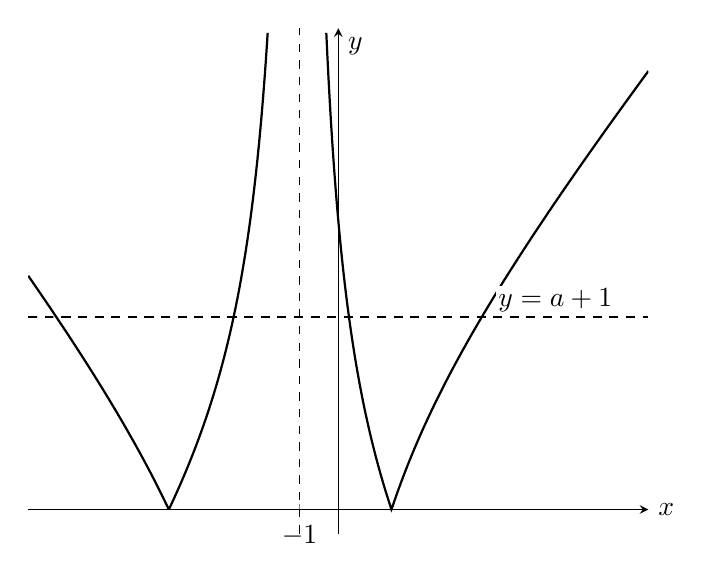
\begin{tikzpicture}
\def\a{3}
\begin{axis}[
  width=0.78\linewidth,
  height=8cm,
  axis lines=middle,
  xmin=-8, xmax=8,
  ymin=-0.5, ymax=10,
  xlabel={$x$},
  ylabel={$y$},
  xtick={-1},
  xticklabels={$-1$},
  ytick=\empty,
  every axis x label/.style={
    at={(current axis.right of origin)},
    anchor=west,
    xshift=0pt
  },
  samples=300,
  clip=true,
  restrict y to domain=-0.5:10,
  unbounded coords=jump
]

  \addplot[dashed] coordinates {(-1,-0.5) (-1,10)};

  \addplot[thick, domain=-8:-1.03] {abs((x^2 + \a*x - 6)/(x + 1))};
  \addplot[thick, domain=-0.97:8]  {abs((x^2 + \a*x - 6)/(x + 1))};

  \addplot[dashed, domain=-8:8] {\a + 1};
  \node[fill=white, inner sep=1pt] at (axis cs:5.6,4.35) {$y=a+1$};
\end{axis}
\end{tikzpicture}

    \item The endpoints of the given intervals are where
    \[
    \left|\frac{x^2+ax-6}{x+1}\right|=a+1
    \]

    From the intervals
    \[
    -11<x<-3 \quad \text{and} \quad 0<x<4
    \]
    we can see that $x=0$ is one boundary point. So
    \[
    \left|\frac{0^2+a(0)-6}{0+1}\right|=a+1
    \]
    \[
    6=a+1
    \]
    \[
    a=5
    \]
  \end{enumerate}
\end{enumerate}
\end{tcolorbox}


\newpage

% ---- Question 6 ----
\questionitem
% [Source: _QBT___Solns__Rational_Functions, Q6]


The function $f$ is defined by
\[
f(x)=\frac{x^2+2x-3}{x^2+px+4} \qquad x \in \mathbb{R}
\]
where $p$ is a constant. \\

The graph of $y=f(x)$ has only one asymptote. \\
\begin{enumerate}[label=\textbf{(\alph*)}]
  \item Write down the equation of the asymptote. \marks{1} \\
  \item Find the set of possible values of $p$. \marks{4} \\
  \item Find the coordinates of the points at which the graph of $y=f(x)$ intersects the coordinate axes. \marks{3} \\

\begin{figure}[H]
    \centering
\begin{tikzpicture}
\pgfmathsetmacro{\xM}{4.5}
\pgfmathsetmacro{\yM}{4/3}
\pgfmathsetmacro{\kval}{0.2}
\begin{axis}[
    axis lines=center,
    xlabel={$x$},
    ylabel={$y$},
    xmin=-7, xmax=7,
    ymin=-1.2, ymax=1.6,
    xtick=\empty,
    ytick=\empty,
    clip=false,
    width=10cm,
    height=6.2cm,
    every axis x label/.style={at={(ticklabel* cs:1)}, anchor=west},
    every axis y label/.style={at={(ticklabel* cs:1)}, anchor=south}
]
\addplot[thick, black, samples=300, domain=-7:7] {(x^2 + 2*x - 3)/(x^2 - x + 4)};
\addplot[dashed, black, samples=2, domain=-7:7] {\kval};
\node[above right] at (axis cs:-7,0.6) {$C$};
\node[above right] at (axis cs:4.5,\kval) {$y=k$};
\node[below left] at (axis cs:0,0) {$O$};
\node[above] at (axis cs:\xM,\yM) {$M$};
\end{axis}
\end{tikzpicture}
\end{figure}

  
  \item A curve $C$ has equation
  \[
  y=\frac{x^2+2x-3}{x^2-x+4}
  \]
  The curve $C$ has a local maximum at the point $M$ as shown in the diagram. \\
  The line $y=k$ intersects curve $C$. \\
  \begin{enumerate}[label=(\roman*)]
    \item Show that
    \[
    15k^2-8k-16 \le 0
    \]
    \marks[-20pt]{5}
    \item Hence, find the $y$-coordinate of point $M$. \marks{2}
  \end{enumerate}
\end{enumerate}

\vspace*{10pt}

\begin{tcolorbox}[colback=white, colframe=scarlet, title={\textbf{Solution}}, breakable, grow to left by=6mm, grow to right by=10mm]
\begin{enumerate}[label=\textbf{(\alph*)}]
  \item The numerator and denominator have the same degree, and both have leading coefficient $1$.

  So the horizontal asymptote is
  \[
  y=1
  \]

  \item From part (a), one asymptote is already $y=1$.

  For the graph to have \emph{only one} asymptote, there must be no vertical asymptotes. Vertical asymptotes would occur if the denominator
  \[
  x^2+px+4
  \]
  had any real roots.

  Therefore we require the quadratic $x^2+px+4=0$ to have no real solutions, so its discriminant must be negative:
  \[
  p^2-4(1)(4)<0
  \]
  \[
  p^2-16<0
  \]
  \[
  p^2<16
  \]
  \[
  -4<p<4
  \]

  \item To find the $x$-intercepts, set $y=0$. Then the numerator must be zero:
  \[
  x^2+2x-3=0
  \]
  \[
  (x+3)(x-1)=0
  \]
  \[
  x=-3 \quad \text{or} \quad x=1
  \]

  So the possible points are $(-3,0)$ and $(1,0)$.

  We must also check the denominator is not zero at these values. Since from part (b), $-4<p<4$,
  \[
  (-3)^2+p(-3)+4=13-3p>1
  \]
  and
  \[
  1^2+p(1)+4=p+5>1
  \]
  so both are non-zero.

  Hence the graph intersects the $x$-axis at
  \[
  (-3,0)\quad \text{and}\quad (1,0)
  \]

  To find the $y$-intercept, set $x=0$:
  \[
  y=\frac{0^2+2(0)-3}{0^2+p(0)+4}=\frac{-3}{4}
  \]

  So the graph intersects the $y$-axis at
  \[
  \left(0,-\frac34\right)
  \]

  \item 
  \begin{enumerate}[label=(\roman*)]
    \item The line $y=k$ intersects the curve
    \[
    y=\frac{x^2+2x-3}{x^2-x+4}
    \]
    when
    \[
    k=\frac{x^2+2x-3}{x^2-x+4}
    \]

    First note that
    \[
    x^2-x+4=\left(x-\frac12\right)^2+\frac{15}{4}>0
    \]
    for all real $x$, so we may multiply through safely.

    Hence
    \[
    x^2+2x-3=k(x^2-x+4)
    \]

    Rearranging,
    \begin{align*}
    x^2+2x-3 &= kx^2-kx+4k \\
    0 &= kx^2-kx+4k-x^2-2x+3 \\
    0 &= (k-1)x^2-(k+2)x+(4k+3)
    \end{align*}

    Equivalently,
    \[
    (1-k)x^2+(2+k)x-(3+4k)=0
    \]

    For the line to intersect the curve, this quadratic in $x$ must have at least one real root. So its discriminant is non-negative:
    \[
    (2+k)^2-4(1-k)\bigl(-(3+4k)\bigr)\ge 0
    \]
    \[
    (2+k)^2+4(1-k)(3+4k)\ge 0
    \]

    Now expand:
    \begin{align*}
    (2+k)^2+4(1-k)(3+4k) &\ge 0 \\
    (k^2+4k+4)+4(3+4k-3k-4k^2) &\ge 0 \\
    k^2+4k+4+4(3+k-4k^2) &\ge 0 \\
    k^2+4k+4+12+4k-16k^2 &\ge 0 \\
    -15k^2+8k+16 &\ge 0
    \end{align*}

    Therefore
    \[
    15k^2-8k-16\le 0
    \]

    as required.

    \item At the local maximum, the horizontal line $y=k$ just touches the curve, so there is exactly one value of $x$. Therefore the discriminant is zero, so
    \[
    15k^2-8k-16=0
    \]

    Solving,
    \[
    k=\frac{8\pm\sqrt{(-8)^2-4(15)(-16)}}{2(15)}
    =\frac{8\pm\sqrt{64+960}}{30}
    =\frac{8\pm 32}{30}
    \]

    So
    \[
    k=\frac{40}{30}=\frac43
    \qquad \text{or} \qquad
    k=\frac{-24}{30}=-\frac45
    \]

    The local maximum has the larger $y$-value, so the $y$-coordinate of $M$ is
    \[
    \frac43
    \]
  \end{enumerate}
\end{enumerate}
\end{tcolorbox}


\newpage

% ---- Question 7 ----
\questionitem
% [Source: _QBT___Solns__Rational_Functions, Q7]

A curve has equation
\[
y = \frac{x^2 - 9}{x^2 - 4}
\]
\begin{enumerate}[label=\textbf{(\alph*)}]
  \item Write down the equations of the asymptotes to the curve. \marks{3} \\
  \item Sketch the curve, indicating the coordinates of the points where the curve intersects the coordinate axes. \marks{5} \\
  \item Hence, or otherwise, solve the inequality
  \[
  0 < \frac{x^2 - 9}{x^2 - 4} < 1
  \]
  \marks[-20pt]{2}
\end{enumerate}

\vspace*{10pt}

\begin{tcolorbox}[colback=white, colframe=scarlet, title={\textbf{Solution}}, breakable, grow to left by=6mm, grow to right by=10mm]
\begin{enumerate}[label=\textbf{(\alph*)}]
  \item Vertical asymptotes occur where the denominator is zero:
  \[
  x^2-4=0
  \]
  so
  \[
  x=\pm 2
  \]

  For large $|x|$, the numerator and denominator have the same degree, so the horizontal asymptote is the ratio of the leading coefficients:
  \[
  y=1
  \]

  Hence the asymptotes are $x=-2$, $x=2$ and $y=1$.

  \item The sketch should look like:

\begin{tikzpicture}
\begin{axis}[
  width=0.8\linewidth,
  height=8.5cm,
  axis lines=middle,
  xmin=-6, xmax=6,
  ymin=-6, ymax=8,
  xlabel={$x$},
  ylabel={$y$},
  xtick={-3,-2,2,3},
  ytick={1,2.25},
  xticklabels={,,,},
  yticklabels={,},
  samples=300,
  clip=true,
  every axis x label/.style={
    at={(current axis.right of origin)},
    anchor=west,
    xshift=0pt
  },
]
  \addplot[dashed] coordinates {(-2,-6) (-2,8)};
  \addplot[dashed] coordinates {(2,-6) (2,8)};
  \addplot[dashed] coordinates {(-6,1) (6,1)};

  \addplot[domain=-6:-2.03, smooth, thick] {(x^2-9)/(x^2-4)};
  \addplot[domain=-1.97:1.97, smooth, thick] {(x^2-9)/(x^2-4)};
  \addplot[domain=2.03:6, smooth, thick] {(x^2-9)/(x^2-4)};

  \node[below=2pt] at (axis cs:-3,0) {$-3$};
  \node[below=2pt, xshift=-8pt] at (axis cs:-1.4,0) {$-2$};
  \node[below=2pt, xshift=8pt] at (axis cs:1.4,0) {$2$};
  \node[below=2pt] at (axis cs:3,0) {$3$};

  \node[left=4pt, yshift=-1pt, fill=white, inner sep=1pt] at (axis cs:0,1) {$1$};
  \node[left=3pt, yshift=4pt, fill=white, inner sep=1pt] at (axis cs:0,2.7) {$\frac94$};
\end{axis}
\end{tikzpicture}

  First write
  \[
  y=\frac{x^2-9}{x^2-4}=1-\frac{5}{x^2-4}
  \]

  Since the equation depends on $x^2$, the curve is symmetric about the $y$-axis.

  The $x$-intercepts are found by setting $y=0$:
  \[
  \frac{x^2-9}{x^2-4}=0 \quad \Rightarrow \quad x^2-9=0
  \]
  so
  \[
  x=\pm 3
  \]
  giving intercepts $(-3,0)$ and $(3,0)$.

  The $y$-intercept is found by setting $x=0$:
  \[
  y=\frac{0-9}{0-4}=\frac94
  \]
  so the point is
  \[
  \left(0,\frac94\right)
  \]

  Also,
  \[
  y=1-\frac{5}{x^2-4}
  \]
  so the curve never meets the line $y=1$.

  For $|x|<2$, we have $x^2-4<0$, so $-\dfrac{5}{x^2-4}>0$ and hence $y>1$.

  For $2<|x|<3$, the numerator is negative and the denominator is positive, so $y<0$.

  For $|x|>3$, both numerator and denominator are positive, so $0<y<1$.

  So the sketch has the correct intercepts and asymptotes as shown.

\item Let
\[
f(x)=\frac{x^2-9}{x^2-4}
\]

From the sketch in part \textbf{(b)}, the inequality
\[
0<f(x)<1
\]
means that the curve must lie \emph{above} the $x$-axis and \emph{below} the horizontal line $y=1$.

Looking at the graph, this happens only on the two outer branches, that is for
\[
x<-3 \quad \text{or} \quad x>3.
\]

Hence the solution to
\[
0<\frac{x^2-9}{x^2-4}<1
\]
is
\[
\boxed{x<-3 \quad \text{or} \quad x>3.}
\]
\end{enumerate}
\end{tcolorbox}


\newpage

% ---- Question 8 ----
\questionitem
% [Source: _QBT___Solns__Rational_Functions, Q8]

The curve $C$ has equation
\[
y=\frac{x^2+3}{x+1}
\]
\begin{enumerate}[label=\textbf{(\alph*)}]
  \item Find the equations of the asymptotes of $C$. \marks{3} \\
  \item Show that there is no point on $C$ for which $-6<y<2$. \marks{4} \\
  \item Sketch $C$. \marks{2} \\
  \item
  \begin{enumerate}[label=(\roman*)]
    \item Sketch the graphs of
    \[
    y=\left|\frac{x^2+3}{x+1}\right| \text{ and } y=|x-1|
    \]
    on the same axes, stating the coordinates of any intersections with the axes. \marks{4}
    \item Use your sketch to find the set of values of $c$ for which
    \[
    \left|\frac{x^2+3}{x+1}\right| \le |x-1|+c
    \]
    has no solution. \marks{1}
  \end{enumerate}
\end{enumerate}

\vspace*{10pt}

\begin{tcolorbox}[colback=white, colframe=scarlet, title={\textbf{Solution}}, breakable, grow to left by=6mm, grow to right by=10mm]
\begin{enumerate}[label=\textbf{(\alph*)}]
  \item Divide the numerator by the denominator:
  \[
  x^2+3=(x+1)(x-1)+4
  \]
  so
  \[
  y=\frac{x^2+3}{x+1}=x-1+\frac{4}{x+1}
  \]

  Hence:
  \begin{itemize}
    \item as $x\to -1$, $\dfrac{4}{x+1}\to \pm\infty$, so there is a vertical asymptote
    \[
    x=-1
    \]
    \item as $x\to \pm\infty$, $\dfrac{4}{x+1}\to 0$, so the curve approaches
    \[
    y=x-1
    \]
  \end{itemize}

  Therefore the asymptotes are $x=-1$ and $y=x-1$.

  \item Start from
  \[
  y=\frac{x^2+3}{x+1}
  \]
  and rearrange:
  \[
  y(x+1)=x^2+3
  \]
  \[
  x^2-yx+(3-y)=0
  \]

  This is a quadratic in $x$. For real values of $x$, its discriminant must satisfy
  \[
  \Delta\ge 0
  \]

  So
  \begin{align*}
  \Delta&=(-y)^2-4(1)(3-y)\\
  &=y^2-12+4y\\
  &=y^2+4y-12\\
  &=(y+6)(y-2)
  \end{align*}

  Hence
  \[
  (y+6)(y-2)\ge 0
  \]

  This gives
  \[
  y\le -6 \quad \text{or} \quad y\ge 2
  \]

  So there is no point on $C$ for which
  \[
  -6<y<2
  \]

  \item The sketch should look like:

  \begin{tikzpicture}
  \begin{axis}[
  width=0.78\linewidth,
  height=8.8cm,
  axis lines=middle,
  xmin=-8, xmax=6,
  ymin=-10, ymax=10,
  xlabel={$x$},
  ylabel={$y$},
  xtick={-1},
  ytick=\empty,
  samples=250,
  clip=true
  ]
  \addplot[dashed, domain=-8:6] {x-1};
  \addplot[dashed] coordinates {(-1,-10) (-1,10)};
  \addplot[thick, domain=-8:-1.05] {(x^2+3)/(x+1)};
  \addplot[thick, domain=-0.95:6] {(x^2+3)/(x+1)};
  \end{axis}
  \end{tikzpicture}

  Finding the y-intercept:
  \[
  y(0)=3
  \]
  so the $y$-intercept is $(0,3)$.

  There is no $x$-intercept because
  \[
  \frac{x^2+3}{x+1}=0 \;\Rightarrow\; x^2+3=0
  \]
  which has no real solution.

  \item
  \begin{enumerate}[label=(\roman*)]
    \item The two sketches should look like:

    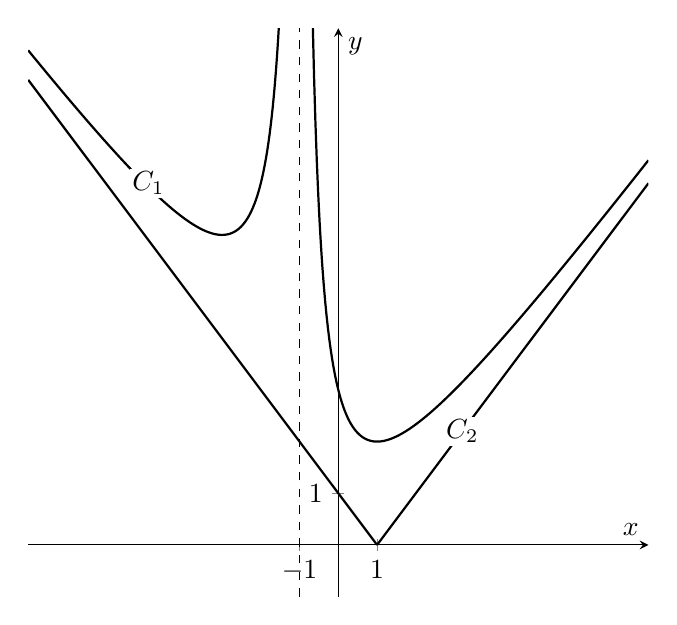
\begin{tikzpicture}
    \begin{axis}[
    width=0.78\linewidth,
    height=8.8cm,
    axis lines=middle,
    xmin=-8, xmax=8,
    ymin=-1, ymax=10,
    xlabel={$x$},
    ylabel={$y$},
    xtick={-1,1},
    ytick={1},
    samples=250,
    clip=true
    ]
    \addplot[dashed] coordinates {(-1,-1) (-1,10)};
    \addplot[thick, domain=-8:-1.05] {-(x^2+3)/(x+1)};
    \addplot[thick, domain=-0.95:8] {(x^2+3)/(x+1)};
    \addplot[thick, domain=-8:1] {1-x};
    \addplot[thick, domain=1:8] {x-1};
    \node[fill=white, inner sep=1pt] at (axis cs:-4.9,7) {$C_1$};
    \node[fill=white, inner sep=1pt] at (axis cs:3.2,2.2) {$C_2$};
    \end{axis}
    \end{tikzpicture}

    Here
    \[
    C_1:\ y=\left|\frac{x^2+3}{x+1}\right|,
    \qquad
    C_2:\ y=|x-1|
    \]

    For $C_1$, the part of the original curve with $x<-1$ is reflected in the $x$-axis.The right-hand branch is unchanged.

    Its intersections with the axes are:
    \[
    y=\left|\frac{0^2+3}{0+1}\right|=3
    \]
    so the $y$-intercept is $(0,3)$.

    There is no $x$-intercept, since $x^2+3>0$ for all real $x$.

    Also, $C_1$ has vertical asymptote $x=-1$, and its oblique asymptotes are
    \[
    y=1-x \quad \text{as } x\to -\infty,
    \qquad
    y=x-1 \quad \text{as } x\to \infty
    \]

    For $C_2:y=|x-1|$:
    \[
    |x-1|=0 \Rightarrow x=1
    \]
    so the $x$-intercept is $(1,0)$, and
    \[
    y=|0-1|=1
    \]
    so the $y$-intercept is $(0,1)$. \\

    \item From the sketch, $y=\left|\dfrac{x^2+3}{x+1}\right|$ lies above $y=|x-1|$ for all $x$, and the gap tends to $0$ as $x\to \pm\infty$.

    For the equality case $c=0$,
    \begin{align*}
    \left|\frac{x^2+3}{x+1}\right|=|x-1|
    &\Rightarrow \frac{(x^2+3)^2}{(x+1)^2}=(x-1)^2\\
    &\Rightarrow (x^2+3)^2=(x-1)^2(x+1)^2\\
    &\Rightarrow (x^2+3)^2=(x^2-1)^2\\
    &\Rightarrow x^4+6x^2+9=x^4-2x^2+1\\
    &\Rightarrow 8x^2+8=0
    \end{align*}
    which is impossible for real $x$.

    So there is no solution when $c=0$, and therefore no solution for any $c<0$ either. Since the graphs get arbitrarily close for large positive or negative $x$, any $c>0$ gives a solution.

    Hence the inequality has no solution for
    \[
    c\le 0
    \]
  \end{enumerate}
\end{enumerate}
\end{tcolorbox}


\newpage

% ---- Question 9 ----
\questionitem
% [Source: _QBT___Solns__Rational_Functions, Q9]

Let $a$ be a positive constant. \\
\begin{enumerate}[label=\textbf{(\alph*)}]
  \item The curve $C_1$ has equation
  \[
  y=\frac{x^2-a^2}{x^2-4a^2}
  \]
  Sketch $C_1$. \marks{2} \\
  \end{enumerate}
  The curve $C_2$ has equation
  \[
  y=\left(\frac{x^2-a^2}{x^2-4a^2}\right)^2
  \]
  The curve $C_3$ has equation
  \[
  y=\left|\frac{x^2-a^2}{x^2-4a^2}\right|
  \]
  \\
  \begin{enumerate}[label=\textbf{(\alph*)}, resume]
  \item
  \begin{enumerate}[label=(\roman*)]
    \item Find the coordinates of all stationary points of $C_2$. \marks{3}
    \item Find also the coordinates of all points of intersection of $C_2$ and $C_3$. \marks{3} \\
  \end{enumerate}
  \item Sketch $C_2$ and $C_3$ on a single diagram, clearly identifying each curve. Hence find the set of values of $x$ for which
  \[
  \left(\frac{x^2-a^2}{x^2-4a^2}\right)^2 \leq \left|\frac{x^2-a^2}{x^2-4a^2}\right|
  \]
  \marks[-30pt]{5}
\end{enumerate}

\vspace*{10pt}

\begin{tcolorbox}[colback=white, colframe=scarlet, title={\textbf{Solution}}, breakable, grow to left by=6mm, grow to right by=10mm]
\begin{enumerate}[label=\textbf{(\alph*)}]
  \item The sketch should look like:
  
  \begin{tikzpicture}
  \begin{axis}[
    axis lines=middle,
    width=0.78\linewidth,
    height=8cm,
    xmin=-4.2, xmax=4.2,
    ymin=-3.5, ymax=3.5,
    xtick={-2,-1,1,2},
    xticklabels={$-2a$,$-a$,$a$,$2a$},
    ytick={0.25,1},
    yticklabels={$\frac14$,$1$},
    xlabel={$x$},
    ylabel={$y$},
    samples=300,
    clip=true
  ]
    \addplot[dashed, domain=-4.2:4.2] {1};
    \addplot[dashed] coordinates {(-2,-3.5) (-2,3.5)};
    \addplot[dashed] coordinates {(2,-3.5) (2,3.5)};
    
    \addplot[thick, domain=-4.2:-2.03] {(x^2-1)/(x^2-4)};
    \addplot[thick, domain=-1.97:1.97] {(x^2-1)/(x^2-4)};
    \addplot[thick, domain=2.03:4.2] {(x^2-1)/(x^2-4)};
    
    \node[fill=white, inner sep=1pt] at (axis cs:3.15,1.45) {$C_1$};
  \end{axis}
  \end{tikzpicture}
  
  Since the equation involves only $x^2$, $C_1$ is even, so it is symmetric about the $y$-axis.

  The vertical asymptotes are where
  \[
  x^2-4a^2=0 \quad \Rightarrow \quad x=\pm 2a
  \]
  and as $x\to\pm\infty$,
  \[
  \frac{x^2-a^2}{x^2-4a^2}\to 1
  \]
  so the horizontal asymptote is $y=1$.

  The intercepts are:
  \[
  y=0 \Rightarrow x^2-a^2=0 \Rightarrow x=\pm a
  \]
  so $(\pm a,0)$, and
  \[
  x=0 \Rightarrow y=\frac{-a^2}{-4a^2}=\frac14
  \]
  so $(0,\tfrac14)$.

  Also, $y>1$ for $|x|>2a$, $y<0$ for $a<|x|<2a$, and $0\le y<1$ for $|x|<a$.

  \item 
  \begin{enumerate}[label=\textbf{(\roman*)}]
    \item Let
    \[
    g(x)=\left(\frac{x^2-a^2}{x^2-4a^2}\right)^2
    \]
    Write
    \[
    f(x)=\frac{x^2-a^2}{x^2-4a^2}
    \]
    so that $g(x)=\bigl(f(x)\bigr)^2$.

    Then
    \[
    g'(x)=2f(x)f'(x)
    \]
    and, using the quotient rule,
    \begin{align*}
    f'(x)
    &=\frac{(2x)(x^2-4a^2)-(x^2-a^2)(2x)}{(x^2-4a^2)^2} \\
    &=\frac{2x\bigl((x^2-4a^2)-(x^2-a^2)\bigr)}{(x^2-4a^2)^2} \\
    &=\frac{2x(-3a^2)}{(x^2-4a^2)^2} \\
    &=-\frac{6a^2x}{(x^2-4a^2)^2}
    \end{align*}

    So
    \begin{align*}
    g'(x)
    &=2\left(\frac{x^2-a^2}{x^2-4a^2}\right)\left(-\frac{6a^2x}{(x^2-4a^2)^2}\right) \\
    &=-\frac{12a^2x(x^2-a^2)}{(x^2-4a^2)^3}
    \end{align*}

    Stationary points occur when $g'(x)=0$, so
    \[
    -12a^2x(x^2-a^2)=0
    \]
    Hence
    \[
    x=0 \quad \text{or} \quad x^2=a^2 \Rightarrow x=\pm a
    \]

    Now find the corresponding $y$-coordinates:
    \[
    g(0)=\left(\frac{-a^2}{-4a^2}\right)^2=\left(\frac14\right)^2=\frac1{16}
    \]
    and
    \[
    g(\pm a)=0
    \]

    Therefore the stationary points are
    \[
    (0,\tfrac1{16}), \quad (-a,0), \quad (a,0)
    \]

    \item The curves $C_2$ and $C_3$ have equations
    \[
    y=\left(\frac{x^2-a^2}{x^2-4a^2}\right)^2
    \qquad \text{and} \qquad
    y=\left|\frac{x^2-a^2}{x^2-4a^2}\right|
    \]

    Let
    \[
    u=\left|\frac{x^2-a^2}{x^2-4a^2}\right|
    \]
    Then intersections satisfy
    \[
    u^2=u
    \]
    so
    \[
    u(u-1)=0
    \]
    Hence
    \[
    u=0 \quad \text{or} \quad u=1
    \]

    If $u=0$, then
    \[
    \left|\frac{x^2-a^2}{x^2-4a^2}\right|=0
    \]
    so
    \[
    x^2-a^2=0 \Rightarrow x=\pm a
    \]
    and then $y=0$.

    So two intersection points are
    \[
    (\pm a,0)
    \]

    If $u=1$, then
    \[
    \left|\frac{x^2-a^2}{x^2-4a^2}\right|=1
    \]
    so
    \[
    \frac{x^2-a^2}{x^2-4a^2}=\pm 1
    \]

    First, if
    \[
    \frac{x^2-a^2}{x^2-4a^2}=1
    \]
    then
    \[
    x^2-a^2=x^2-4a^2
    \]
    which gives
    \[
    -a^2=-4a^2
    \]
    impossible.

    Next, if
    \[
    \frac{x^2-a^2}{x^2-4a^2}=-1
    \]
    then
    \begin{align*}
    x^2-a^2&=-(x^2-4a^2) \\
    x^2-a^2&=-x^2+4a^2 \\
    2x^2&=5a^2 \\
    x^2&=\frac{5a^2}{2}
    \end{align*}
    so
    \[
    x=\pm a\sqrt{\frac52}
    \]
    and since $u=1$,
    \[
    y=1
    \]

    Therefore the points of intersection are
    \[
    (\pm a,0), \quad \left(\pm a\sqrt{\frac52},1\right)
    \]
  \end{enumerate} \newpage

  \item The sketch should look like:
  
  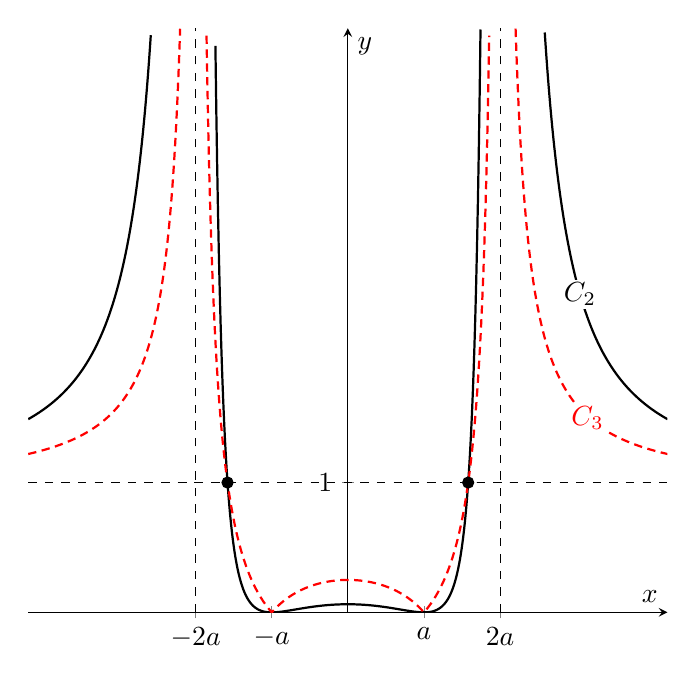
\begin{tikzpicture}
\begin{axis}[
  axis lines=middle,
  width=0.8\linewidth,
  height=9cm,
  xmin=-4.2, xmax=4.2,
  ymin=0, ymax=4.5,
  xtick={-2,-1,1,2},
  xticklabels={$-2a$,$-a$,$a$,$2a$},
  ytick={1},
  yticklabels={$1$},
  xlabel={$x$},
  ylabel={$y$},
  samples=350,
  clip=true,
  restrict y to domain=0:4.5,
  unbounded coords=jump
]
  \addplot[dashed, domain=-4.2:4.2] {1};
  \addplot[dashed] coordinates {(-2,0) (-2,4.5)};
  \addplot[dashed] coordinates {(2,0) (2,4.5)};
  
  \addplot[thick, domain=-4.2:-2.03] {((x^2-1)/(x^2-4))^2};
  \addplot[thick, domain=-1.99:1.97] {((x^2-1)/(x^2-4))^2};
  \addplot[thick, domain=2.01:4.2] {((x^2-1)/(x^2-4))^2};
  
\addplot[thick, densely dashed, red, domain=-4.2:-2.03] {abs((x^2-1)/(x^2-4))};
\addplot[thick, densely dashed, red, domain=-1.97:1.97] {abs((x^2-1)/(x^2-4))};
\addplot[thick, densely dashed, red, domain=2.03:4.2] {abs((x^2-1)/(x^2-4))};

\node[text=red, fill=white, inner sep=1pt] at (axis cs:3.15,1.5) {$C_3$};
  
  \addplot[only marks, mark=*] coordinates {
    (-1.5811,1) (1.5811,1)
  };
  
  \node[fill=white, inner sep=1pt] at (axis cs:3.05,2.45) {$C_2$};
\end{axis}
\end{tikzpicture}
  
  Both curves are even, so both are symmetric about the $y$-axis.

  They have the same vertical asymptotes $x=\pm 2a$ and the same horizontal asymptote $y=1$.

  From part (b)(i), $C_2$ has stationary points
  \[
  (0,\tfrac1{16}), \quad (\pm a,0)
  \]
  and from part (b)(ii), the curves meet at
  \[
  (\pm a,0), \quad \left(\pm a\sqrt{\frac52},1\right)
  \]

  Also, $C_3=\left|C_1\right|$, so it passes through $(0,\tfrac14)$ and has cusps at $(\pm a,0)$.

  From the sketch, $C_2$ lies below or on $C_3$ between the outer intersection points. Therefore
  \[
  \left(\frac{x^2-a^2}{x^2-4a^2}\right)^2 \le \left|\frac{x^2-a^2}{x^2-4a^2}\right|
  \]
  for
  \[
  -a\sqrt{\frac52}\le x\le a\sqrt{\frac52}
  \]

  So the required set of values is
  \[
  -a\sqrt{\frac52}\le x\le a\sqrt{\frac52}
  \]
\end{enumerate}
\end{tcolorbox}


\newpage

% ---- Question 10 ----
\questionitem
% [Source: _QBT___Solns__Rational_Functions, Q10]

A curve $C_1$ has equation
\[
y=-2+\frac{12}{x+3}
\]

\begin{enumerate}[label=\textbf{(\alph*)}]
  \item Write down the equations of the asymptotes of curve $C_1$. \marks{2} \\
  \item Sketch the graph of curve $C_1$. 
  Indicate the values of the intercepts of the curve with the axes. \marks{3}
  \item Hence, or otherwise, solve the inequality
  \[
  -2+\frac{12}{x+3}>0
  \]
  \marks[-20pt]{2}
  \item Curve $C_2$ is a reflection of curve $C_1$ in the line $y=-x$.
  Find an equation for curve $C_2$ in the form $y=f(x)$. \marks{3}
\end{enumerate}

\vspace*{10pt}

\begin{tcolorbox}[colback=white, colframe=scarlet, title={\textbf{Solution}}, breakable, grow to left by=6mm, grow to right by=10mm]
\begin{enumerate}[label=\textbf{(\alph*)}]
  \item For
  \[
  y=-2+\frac{12}{x+3}
  \]
  the denominator is zero when \(x+3=0\), so the vertical asymptote is
  \[
  x=-3
  \]
  Also, as \(x\to \pm\infty\),
  \[
  \frac{12}{x+3}\to 0
  \]
  so
  \[
  y\to -2
  \]
  Hence the horizontal asymptote is
  \[
  y=-2
  \]

  Therefore the asymptotes are \(x=-3\) and \(y=-2\).

  \item The sketch should look like:

  \begin{tikzpicture}
  \begin{axis}[
      axis lines=center,
      xlabel={$x$},
      ylabel={$y$},
      xmin=-10, xmax=10,
      ymin=-10, ymax=10,
      xtick={-3,3},
      ytick={-2,2},
      width=0.8\linewidth,
      height=8.5cm,
      clip=true,
      every axis x label/.style={at={(ticklabel* cs:1)}, anchor=west},
      every axis y label/.style={at={(ticklabel* cs:1)}, anchor=south west},
  ]
  \addplot[dashed, black] coordinates {(-3,-10) (-3,10)};
  \addplot[dashed, black] coordinates {(-10,-2) (10,-2)};
  \addplot[thick, black, samples=200, domain=-10:-3.15] {-2 + 12/(x+3)};
  \addplot[thick, black, samples=200, domain=-2.85:10] {-2 + 12/(x+3)};
  \node[below left] at (axis cs:0,0) {$O$};
  \node[fill=white, inner sep=1pt] at (axis cs:4.8,-0.6) {$C_1$};
  \end{axis}
  \end{tikzpicture}

  This is a rectangular hyperbola with centre \((-3,-2)\), with asymptotes \(x=-3\) and \(y=-2\).  
  For \(x>-3\), the branch lies above \(y=-2\); for \(x<-3\), the branch lies below \(y=-2\).

  To find the intercepts:

  Setting \(x=0\),
  \[
  y=-2+\frac{12}{0+3}=-2+4=2
  \]
  so the \(y\)-intercept is \((0,2)\).

  Setting \(y=0\),
  \begin{align*}
  -2+\frac{12}{x+3}&=0\\
  2x&=6\\
  x&=3
  \end{align*}
  so the \(x\)-intercept is \((3,0)\).

  Therefore the intercepts are \((3,0)\) and \((0,2)\).

\item We need to solve
\[
-2+\frac{12}{x+3}>0
\]

From the sketch in part \textbf{(b)}, this means we want the part of the curve that lies \emph{above} the $x$-axis.

Looking at the graph, curve $C_1$ is above the $x$-axis only between its vertical asymptote at $x=-3$ and its $x$-intercept at $x=3$.

  Hence
  \[
  -3<x<3
  \]

  \item Reflection in the line \(y=-x\) maps each point \((x,y)\) to \((-y,-x)\).

  So in the equation of \(C_1\), replace \(x\) by \(-y\) and \(y\) by \(-x\):
  \[
  -x=-2+\frac{12}{-y+3}
  \]
  that is,
  \[
  -x=-2+\frac{12}{3-y}
  \]

  Now solve for \(y\):
  \begin{align*}
  -x+2&=\frac{12}{3-y}\\
  3-y&=\frac{12}{2-x}
  \end{align*}

  Since \(2-x=-(x-2)\),
  \[
  \frac{12}{2-x}=-\frac{12}{x-2}
  \]
  so
  \begin{align*}
  3-y&=-\frac{12}{x-2}\\[5pt]
  y&=3+\frac{12}{x-2}
  \end{align*}

Hence the equation of $C_2$ is 
\[
y=3+\frac{12}{x-2}
\]

\end{enumerate}
\end{tcolorbox}


\newpage

% ---- Question 11 ----
\questionitem
% [Source: _QBT___Solns__Rational_Functions, Q11]

The curve $C$ has equation
\[
y=\frac{x^2-6x+5}{x+2}
\] \\
\begin{enumerate}[label=\textbf{(\alph*)}]
  \item Find the equations of the asymptotes of $C$. \marks{3} \\
  \item Find the exact coordinates of the stationary points on $C$. \marks{4} \\
  \item Sketch $C$, stating the coordinates of any intersections with the axes. \marks{3} \\
  \item Sketch the curve with equation
  \[
  y=\left|\frac{x^2-6x+5}{x+2}\right|
  \] \\
  and find in exact form the set of values of $x$ for which
  \[
  \left|\frac{x^2-6x+5}{x+2}\right|<6
  \]
  \marks[-30pt]{5}
\end{enumerate}

\vspace*{10pt}

\begin{tcolorbox}[colback=white, colframe=scarlet, title={\textbf{Solution}}, breakable, grow to left by=6mm, grow to right by=10mm]
\begin{enumerate}[label=\textbf{(\alph*)}]
  \item Divide the numerator by the denominator:
  \[
  x^2-6x+5=(x+2)(x-8)+21
  \]
  so
  \[
  y=\frac{x^2-6x+5}{x+2}=x-8+\frac{21}{x+2}
  \]

  From this form:

  \begin{itemize}
    \item the denominator is zero when \(x=-2\), so there is a vertical asymptote
    \[
    x=-2
    \]
    \item as \(x\to \pm\infty\), \(\dfrac{21}{x+2}\to 0\), so the curve approaches
    \[
    y=x-8
    \]
  \end{itemize}

  Hence the asymptotes are \(x=-2\) and \(y=x-8\).

  \item Using
  \[
  y=x-8+\frac{21}{x+2}
  \]
  differentiate:
  \[
  \frac{\mathrm{d}y}{\mathrm{d}x}=1-21(x+2)^{-2}=1-\frac{21}{(x+2)^2}
  \]

  At a stationary point, \(\dfrac{\mathrm{d}y}{\mathrm{d}x}=0\), so
  \begin{align*}
  1-\frac{21}{(x+2)^2}&=0 \\
  \frac{21}{(x+2)^2}&=1 \\
  (x+2)^2&=21 \\
  x+2&=\pm\sqrt{21}
  \end{align*}
  Hence
  \[
  x=-2\pm \sqrt{21}
  \]

  Now find the corresponding \(y\)-coordinates from
  \[
  y=x-8+\frac{21}{x+2}
  \]

  If \(x=-2-\sqrt{21}\), then \(x+2=-\sqrt{21}\), so
  \begin{align*}
  y&=(-2-\sqrt{21})-8+\frac{21}{-\sqrt{21}} \\
   &=-10-\sqrt{21}-\sqrt{21} \\
   &=-10-2\sqrt{21}
  \end{align*}

  If \(x=-2+\sqrt{21}\), then \(x+2=\sqrt{21}\), so
  \begin{align*}
  y&=(-2+\sqrt{21})-8+\frac{21}{\sqrt{21}} \\
   &=-10+\sqrt{21}+\sqrt{21} \\
   &=-10+2\sqrt{21}
  \end{align*}

  So the stationary points are
  \[
  (-2-\sqrt{21},\,-10-2\sqrt{21})
  \quad\text{and}\quad
  (-2+\sqrt{21},\,-10+2\sqrt{21})
  \]

  To identify them, differentiate again:
  \[
  \frac{\mathrm{d}^2y}{\mathrm{d}x^2}=\frac{42}{(x+2)^3}
  \]

  At \(x=-2-\sqrt{21}\), \((x+2)^3<0\), so \(\dfrac{\mathrm{d}^2y}{\mathrm{d}x^2}<0\): this is a local maximum.

  At \(x=-2+\sqrt{21}\), \((x+2)^3>0\), so \(\dfrac{\mathrm{d}^2y}{\mathrm{d}x^2}>0\): this is a local minimum.

  Hence the stationary points are a local maximum at \((-2-\sqrt{21},-10-2\sqrt{21})\) and a local minimum at \((-2+\sqrt{21},-10+2\sqrt{21})\).

  \item The sketch should look like:

  \begin{tikzpicture}
  \begin{axis}[
    axis lines=middle,
    width=0.78\linewidth,
    height=8.5cm,
    xmin=-10, xmax=10,
    ymin=-35, ymax=25,
    xlabel={$x$},
    ylabel={$y$},
    xtick={1, 5},
    ytick={2.5},
    yticklabel={$\frac52$},
    enlargelimits=false,
    clip=true,
    every axis x label/.style={
    at={(current axis.right of origin)},
    anchor=west,
    xshift=0pt
  },
  ]
    \addplot[domain=-10:-2.05, samples=300, smooth] {(x^2-6*x+5)/(x+2)};
    \addplot[domain=-1.95:10, samples=300, smooth] {(x^2-6*x+5)/(x+2)};
    \addplot[dashed, domain=-10:10] {x-8};
    \addplot[dashed] coordinates {(-2,-35) (-2,25)};
    \node[fill=white, inner sep=1pt] at (axis cs:-3.5,8) {$x=-2$};
    \node[fill=white, inner sep=1pt] at (axis cs:7,-3.5) {$y=x-8$};
    \node[fill=white, inner sep=1pt] at (axis cs:7,5) {$C$};
  \end{axis}
  \end{tikzpicture}

  For the intersections with the axes:

  For the \(x\)-axis, set \(y=0\):
  \begin{align*}
  \frac{x^2-6x+5}{x+2}&=0 \\
  x^2-6x+5&=0 \\
  (x-1)(x-5)&=0
  \end{align*}
  So the curve meets the \(x\)-axis at
  \[
  (1,0)\quad\text{and}\quad(5,0)
  \]

  For the \(y\)-axis, set \(x=0\):
  \[
  y=\frac{0^2-6(0)+5}{0+2}=\frac52
  \]
  so the curve meets the \(y\)-axis at
  \[
  \left(0,\frac52\right)
  \]

  The left-hand branch lies below the \(x\)-axis for \(x<-2\), and the right-hand branch falls from \(+\infty\), crosses at \((1,0)\), reaches the minimum found in part (b), then rises through \((5,0)\).

  \item The sketch should look like:

  \begin{tikzpicture}
  \begin{axis}[
    axis lines=middle,
    width=0.78\linewidth,
    height=8.5cm,
    xmin=-10, xmax=10,
    ymin=-5, ymax=40,
    xlabel={$x$},
    ylabel={$y$},
    xtick={1, 5},
    ytick={2.5},
    yticklabel={$\frac52$},
    enlargelimits=false,
    clip=true,
    every axis x label/.style={
    at={(current axis.right of origin)},
    anchor=west,
    xshift=0pt
  },
  ]
    \addplot[domain=-10:-2.05, samples=300, smooth] {abs((x^2-6*x+5)/(x+2))};
    \addplot[domain=-1.95:10, samples=300, smooth] {abs((x^2-6*x+5)/(x+2))};
    \addplot[dashed] coordinates {(-2,-5) (-2,40)};
    \node[fill=white, inner sep=1pt] at (axis cs:-3.5,8.5) {$x=-2$};
  \end{axis}
  \end{tikzpicture}

  For \(y=\left|\dfrac{x^2-6x+5}{x+2}\right|\), every part of the graph of \(C\) below the \(x\)-axis is reflected in the \(x\)-axis. So:

  \begin{itemize}
    \item the whole left-hand branch is reflected above the \(x\)-axis
    \item the part of the right-hand branch between \(x=1\) and \(x=5\) is reflected above the \(x\)-axis
    \item the points \((1,0)\) and \((5,0)\) stay on the curve
    \item \(x=-2\) remains a vertical asymptote
  \end{itemize}

  Now solve
  \[
  \left|\frac{x^2-6x+5}{x+2}\right|<6
  \]

  Since both sides are non-negative, we may square:
  \[
  \frac{(x^2-6x+5)^2}{(x+2)^2}<36
  \]

  For \(x\neq -2\), \((x+2)^2>0\), so multiplying through gives
  \[
  (x^2-6x+5)^2<36(x+2)^2
  \]

  Rearranging as a difference of two squares:
  \begin{align*}
  (x^2-6x+5)^2-36(x+2)^2&<0 \\
  \bigl((x^2-6x+5)-6(x+2)\bigr)\bigl((x^2-6x+5)+6(x+2)\bigr)&<0 \\
  (x^2-12x-7)(x^2+17)&<0
  \end{align*}

  But \(x^2+17>0\) for all real \(x\), so we need
  \[
  x^2-12x-7<0
  \]

  Solve \(x^2-12x-7=0\):
  \begin{align*}
  x&=\frac{12\pm\sqrt{(-12)^2-4(1)(-7)}}{2} \\
   &=\frac{12\pm\sqrt{144+28}}{2} \\
   &=\frac{12\pm\sqrt{172}}{2} \\
   &=6\pm\sqrt{43}
  \end{align*}

  Since the quadratic opens upwards, it is negative between its roots. Therefore
  \[
  6-\sqrt{43}<x<6+\sqrt{43}
  \]

  So the required set of values is \(6-\sqrt{43}<x<6+\sqrt{43}\).
\end{enumerate}
\end{tcolorbox}


\newpage

% ---- Question 12 ----
\questionitem
% [Source: _QBT___Solns__Rational_Functions, Q12]

A curve has equation $y=\dfrac{x-1}{x^2-x-6}$. \\
\begin{enumerate}[label=\textbf{(\alph*)}]
  \item
  \begin{enumerate}[label=(\roman*)]
    \item Write down the equations of the three asymptotes of the curve. \marks{3}
    \item Sketch the curve, showing the coordinates of any points of intersection with the coordinate axes. \marks[-10pt]{4} \\
  \end{enumerate}
  \item Hence, or otherwise, solve the inequality
  \[
  \frac{x-1}{x^2-x-6}>\frac{1}{2}
  \]
  \marks[-20pt]{3}
\end{enumerate}

\vspace*{10pt}

\begin{tcolorbox}[colback=white, colframe=scarlet, title={\textbf{Solution}}, breakable, grow to left by=6mm, grow to right by=10mm]
\begin{enumerate}[label=\textbf{(\alph*)}]
  \item
  \begin{enumerate}[label=\textbf{(\roman*)}]
    \item Factorising the denominator,
    \[
    x^2-x-6=(x-3)(x+2)
    \]
    So the vertical asymptotes are
    \[
    x=3 \quad \text{and} \quad x=-2
    \]
    Since the degree of the denominator is greater than the degree of the numerator, the horizontal asymptote is
    \[
    y=0
    \]
    Hence the three asymptotes are $x=-2$, $x=3$ and $y=0$.

    \item The sketch should look like:

    \begin{tikzpicture}
    \begin{axis}[
      width=0.78\linewidth,
      height=8.5cm,
      axis lines=middle,
      xmin=-6, xmax=6,
      ymin=-5, ymax=5,
      xlabel={$x$},
      ylabel={$y$},
      xtick={-2,1,3},
      ytick={0.1666667},
      yticklabels={$ \frac16 $},
      yticklabel style={xshift=1pt, yshift=9pt},
      every axis x label/.style={
        at={(current axis.right of origin)},
        anchor=west,
        xshift=3pt
      },
      clip=true
    ]
    \addplot[thick, smooth, domain=-6:-2.05, samples=200] {(x-1)/(x^2-x-6)};
    \addplot[thick, smooth, domain=-1.95:2.95, samples=200] {(x-1)/(x^2-x-6)};
    \addplot[thick, smooth, domain=3.05:6, samples=200] {(x-1)/(x^2-x-6)};
    \addplot[dashed] coordinates {(-2,-5) (-2,5)};
    \addplot[dashed] coordinates {(3,-5) (3,5)};
    \end{axis}
    \end{tikzpicture}

    The intersections with the axes are found as follows.

    For the $x$-axis, $y=0$, so
    \[
    x-1=0
    \]
    giving $x=1$. Hence the curve crosses the $x$-axis at $(1,0)$.

    For the $y$-axis, $x=0$, so
    \[
    y=\frac{0-1}{0^2-0-6}=\frac{-1}{-6}=\frac16
    \]
    Hence the curve crosses the $y$-axis at $\left(0,\frac16\right)$.

    Also, as $x\to\pm\infty$, $y\to 0$, so the curve approaches the asymptote $y=0$.
    As $x\to -2^{-}$, $y\to -\infty$ and as $x\to -2^{+}$, $y\to +\infty$.
    As $x\to 3^{-}$, $y\to -\infty$ and as $x\to 3^{+}$, $y\to +\infty$.
    This gives the three branches shown in the sketch. 
  \end{enumerate} \newpage

\item To solve
\[
\frac{x-1}{x^2-x-6}>\frac12
\]
we compare the curve from part \textbf{(a)(ii)} with the line
\[
y=\frac12
\]

First find where the curve meets this line:
\begin{align*}
\frac{x-1}{x^2-x-6}&=\frac12\\
2(x-1)&=x^2-x-6\\
x^2-3x-4&=0\\
(x-4)(x+1)&=0
\end{align*}
So the graphs intersect when
\[
x=-1 \quad \text{or} \quad x=4
\]

\begin{tikzpicture}
\begin{axis}[
  width=0.78\linewidth,
  height=8.5cm,
  axis lines=middle,
  xmin=-6, xmax=6,
  ymin=-5, ymax=5,
  xlabel={$x$},
  ylabel={$y$},
  xtick={-2,-1,1,3,4},
  ytick=\empty,
  every axis x label/.style={
    at={(current axis.right of origin)},
    anchor=west,
    xshift=3pt
  },
  clip=true
]
\addplot[thick, smooth, domain=-6:-2.05, samples=200] {(x-1)/(x^2-x-6)};
\addplot[thick, smooth, domain=-1.95:2.95, samples=200] {(x-1)/(x^2-x-6)};
\addplot[thick, smooth, domain=3.05:6, samples=200] {(x-1)/(x^2-x-6)};
\addplot[dashed] coordinates {(-2,-5) (-2,5)};
\addplot[dashed] coordinates {(3,-5) (3,5)};
\addplot[dashed, red, domain=-6:6] {0.5};
\node[text=red, fill=white, inner sep=1pt] at (axis cs:-4.9,1) {$y=\frac12$};
\end{axis}
\end{tikzpicture}

From the graph, the curve lies above the line $y=\frac12$ for
\[
-2<x<-1
\quad \text{and} \quad
3<x<4
\]

Hence the solution is
\[ 
x\in(-2,-1)\cup(3,4)
\]
\end{enumerate}
\end{tcolorbox}


\newpage

% ---- Question 13 ----
\questionitem
% [Source: _QBT___Solns__Rational_Functions, Q13]

The curve $C$ has equation
\[
y=\frac{(x-1)(x+3)}{x^2-2x+3}
\] \\
\begin{enumerate}[label=\textbf{(\alph*)}]
  \item Show that $C$ has no vertical asymptotes and state the equation of the horizontal asymptote of $C$. \marks{3} \\
  \item Find the coordinates of the stationary points on $C$. \marks{4} \\
  \item Sketch $C$, stating the coordinates of the intersections with the axes. \marks{3} \\
  \item Sketch the curve with equation
  \[
  y=\left|\frac{(x-1)(x+3)}{x^2-2x+3}\right|
  \] \\
  and state the set of values of $k$ for which
  \[
  \left|\frac{(x-1)(x+3)}{x^2-2x+3}\right|=k
  \]
  has $4$ distinct real solutions. \marks{2} \\
\end{enumerate}

\vspace*{10pt}

\begin{tcolorbox}[colback=white, colframe=scarlet, title={\textbf{Solution}}, breakable, grow to left by=6mm, grow to right by=10mm]
\begin{enumerate}[label=\textbf{(\alph*)}]
  \item Write the denominator as
  \[
  x^2-2x+3=(x-1)^2+2
  \]
  Since $(x-1)^2+2>0$ for all real $x$, the denominator is never $0$.

  So $C$ has no vertical asymptotes.

  The numerator and denominator are both quadratic, with the same leading coefficient $1$, so as $x\to \pm \infty$,
  \[
  y \to 1
  \]
  Hence the horizontal asymptote is
  \[
  y=1
  \]

  \item First expand the numerator:
  \[
  y=\frac{(x-1)(x+3)}{x^2-2x+3}=\frac{x^2+2x-3}{x^2-2x+3}
  \]

  Differentiate using the quotient rule:
  \begin{align*}
  \frac{\mathrm{d}y}{\mathrm{d}x}
  &=\frac{(2x+2)(x^2-2x+3)-(x^2+2x-3)(2x-2)}{(x^2-2x+3)^2} \\
  &=\frac{(2x^3-2x^2+2x+6)-(2x^3+2x^2-10x+6)}{(x^2-2x+3)^2} \\
  &=\frac{-4x^2+12x}{(x^2-2x+3)^2} \\
  &=\frac{4x(3-x)}{(x^2-2x+3)^2}
  \end{align*}

  For stationary points, set $\dfrac{\mathrm{d}y}{\mathrm{d}x}=0$.

  Since $(x^2-2x+3)^2>0$ for all $x$, this gives
  \[
  4x(3-x)=0
  \]
  So
  \[
  x=0 \quad \text{or} \quad x=3
  \]

  Now find the corresponding $y$-coordinates:
  \[
  y(0)=\frac{(-1)(3)}{3}=-1
  \]
  \[
  y(3)=\frac{(2)(6)}{6}=2
  \]

  So the stationary points are
  \[
  (0,-1) \quad \text{and} \quad (3,2)
  \]

  Also, since the sign of $\dfrac{\mathrm{d}y}{\mathrm{d}x}$ is the sign of $x(3-x)$, it is negative for $x<0$, positive for $0<x<3$, and negative for $x>3$.

  Therefore $(0,-1)$ is a minimum point and $(3,2)$ is a maximum point.

  \item The sketch should look like:

  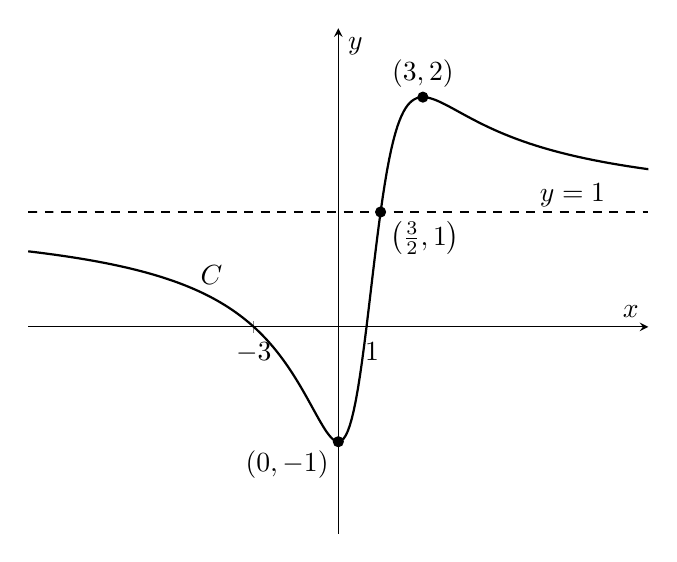
\begin{tikzpicture}
 \begin{axis}[
  width=0.78\linewidth,
  height=8cm,
  axis lines=middle,
  xlabel={$x$},
  ylabel={$y$},
  xmin=-11, xmax=11,
  ymin=-1.8, ymax=2.6,
  xtick={-3},
  xticklabels={$-3$},
  extra x ticks={1},
  extra x tick labels={$1$},
  extra x tick style={
    tick label style={xshift=2pt}
  },
  ytick=\empty,
  domain=-11:11,
  samples=300,
  clip=true
]
  \addplot[black, thick] {((x-1)*(x+3))/(x^2-2*x+3)};
  \addplot[black, dashed] {1};
  \addplot[only marks, mark=*, mark size=1.8pt] coordinates {(0,-1) (3,2) (1.5,1)};
  \node[left] at (axis cs:0,-1.2) {$(0,-1)$};
  \node[above] at (axis cs:3,2) {$(3,2)$};
  \node[below right] at (axis cs:1.5,1) {$\left(\frac32,1\right)$};
  \node[right] at (axis cs:6.8,1.15) {$y=1$};
  \node[fill=white, inner sep=1pt] at (axis cs:-4.5,0.45) {$C$};
  \end{axis}
  \end{tikzpicture}

  Intersections with the $x$-axis occur when $y=0$, so the numerator must be $0$:
  \[
  (x-1)(x+3)=0
  \]
  Hence
  \[
  x=1 \quad \text{or} \quad x=-3
  \]
  So the $x$-intercepts are
  \[
  (1,0) \quad \text{and} \quad (-3,0)
  \]

  The intersection with the $y$-axis is found by putting $x=0$:
  \[
  y=\frac{(-1)(3)}{3}=-1
  \]
  So the $y$-intercept is
  \[
  (0,-1)
  \]

  Using parts (a) and (b), the curve is continuous for all $x$, has horizontal asymptote $y=1$, minimum point $(0,-1)$ and maximum point $(3,2)$.

  It also crosses the horizontal asymptote when $y=1$:
  \[
  \frac{x^2+2x-3}{x^2-2x+3}=1
  \]
  \[
  x^2+2x-3=x^2-2x+3
  \]
  \[
  4x=6
  \]
  \[
  x=\frac32
  \]
  So it crosses the asymptote at
  \[
  \left(\frac32,1\right)
  \]

\item The sketch should look like:

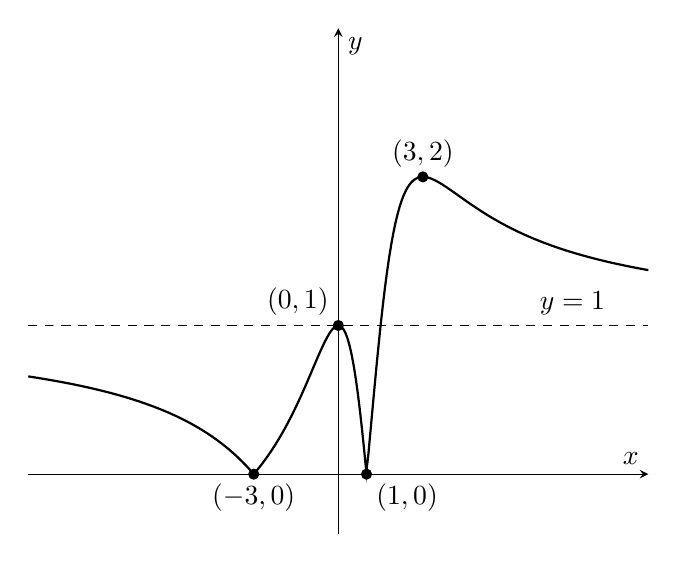
\begin{tikzpicture}
\begin{axis}[
width=0.78\linewidth,
height=8cm,
axis lines=middle,
xlabel={$x$},
ylabel={$y$},
xmin=-11, xmax=11,
ymin=-0.4, ymax=3,
xtick=\empty, ytick=\empty,
domain=-11:11,
samples=300,
clip=true
]
\addplot[black, thick] {abs(((x-1)*(x+3))/(x^2-2*x+3))};
\addplot[black, dashed] {1};
\addplot[only marks, mark=*, mark size=1.8pt] coordinates {(-3,0) (1,0) (0,1) (3,2)};
\node[below] at (axis cs:-3,0) {$(-3,0)$};
\node[below right] at (axis cs:1,0) {$(1,0)$};
\node[above left] at (axis cs:0,1) {$(0,1)$};
\node[above] at (axis cs:3,2) {$(3,2)$};
\node[right] at (axis cs:6.8,1.15) {$y=1$};
\end{axis}
\end{tikzpicture}

To solve
\[
\left|\frac{(x-1)(x+3)}{x^2-2x+3}\right|=k,
\]
draw the horizontal line $y=k$.

For there to be $4$ distinct real solutions, the line must meet the curve four times: once on the left-hand branch, twice on the middle arch, and once on the right-hand branch.\\

From the sketch, this happens exactly when the line lies above the $x$-axis and below the point $(0,1)$, that is,
\[
0<k<1
\]

Hence the required set of values is
\[
\boxed{0<k<1}
\]
\end{enumerate}
\end{tcolorbox}


\newpage

% ---- Question 14 ----
\questionitem
% [Source: _QBT___Solns__Rational_Functions, Q14]

The curve $C$ has equation
\[
y=\dfrac{-x^2+4x+5}{x+2}
\] \\
\begin{enumerate}[label=\textbf{(\alph*)}]
  \item Find the equations of the asymptotes of $C$. \marks{3} \\
  \item Find the coordinates of the stationary points of $C$. \marks{4} \\
  \item Sketch $C$, stating the coordinates of the intersections with the axes. \marks{3} \\
  \item Sketch the curve with equation
  \[
  y=\left|\dfrac{-x^2+4x+5}{x+2}\right|
  \]
  \marks[-20pt]{2}
  \item Using your sketch, or otherwise, find the set of values of $x$ for which
  \[
  \left|\dfrac{-x^2+4x+5}{x+2}\right|<2
  \]
  \marks[-30pt]{4}
\end{enumerate}

\vspace*{10pt}

\begin{tcolorbox}[colback=white, colframe=scarlet, title={\textbf{Solution}}, breakable, grow to left by=6mm, grow to right by=10mm]
\begin{enumerate}[label=\textbf{(\alph*)}]
  \item Divide the numerator by $x+2$:
  \begin{align*}
  -x^2+4x+5&=(-x+6)(x+2)-7
  \end{align*}
  so
  \[
  y=-x+6-\frac{7}{x+2}
  \]

  Hence the denominator is zero when $x=-2$, so there is a vertical asymptote
  \[
  x=-2
  \]

  Also, as $x\to\pm\infty$, the term $\dfrac{-7}{x+2}\to 0$, so the oblique asymptote is
  \[
  y=-x+6
  \]

  Therefore the asymptotes are $x=-2$ and $y=-x+6$.

  \item Using
  \[
  y=-x+6-\frac{7}{x+2}
  \]
  differentiate:
  \[
  \frac{\mathrm{d}y}{\mathrm{d}x}=-1+\frac{7}{(x+2)^2}
  \]

  At a stationary point,
  \[
  -1+\frac{7}{(x+2)^2}=0
  \]
  so
  \begin{align*}
  \frac{7}{(x+2)^2}&=1\\
  (x+2)^2&=7\\
  x+2&=\pm\sqrt7\\
  x&=-2\pm\sqrt7
  \end{align*}

  Now find the corresponding $y$-values.

  For $x=-2-\sqrt7$:
  \begin{align*}
  y&=-(-2-\sqrt7)+6-\frac{7}{-\sqrt7}\\
   &=2+\sqrt7+6+\sqrt7\\
   &=8+2\sqrt7
  \end{align*}

  For $x=-2+\sqrt7$:
  \begin{align*}
  y&=-(-2+\sqrt7)+6-\frac{7}{\sqrt7}\\
   &=2-\sqrt7+6-\sqrt7\\
   &=8-2\sqrt7
  \end{align*}

  To classify them, differentiate again:
  \[
  \frac{\mathrm{d}^2y}{\mathrm{d}x^2}=-\frac{14}{(x+2)^3}
  \]

  At $x=-2-\sqrt7$, $(x+2)=-\sqrt7$, so $\dfrac{\mathrm{d}^2y}{\mathrm{d}x^2}>0$ and this is a minimum.

  At $x=-2+\sqrt7$, $(x+2)=\sqrt7$, so $\dfrac{\mathrm{d}^2y}{\mathrm{d}x^2}<0$ and this is a maximum.

  Therefore the stationary points are
  \[
  (-2-\sqrt7,\ 8+2\sqrt7)\quad\text{and}\quad(-2+\sqrt7,\ 8-2\sqrt7)
  \]
  with the first a minimum and the second a maximum.

  \item Using the asymptotes and stationary points from earlier parts, the sketch should look like:

\begin{tikzpicture}
\begin{axis}[
  axis lines=middle,
  xlabel={$x$},
  ylabel={$y$},
  xmin=-12, xmax=8,
  ymin=-10, ymax=24,
  width=0.80\linewidth,
  height=8.8cm,
  xtick={-1, 5},
  ytick={2.5},
  yticklabels={$\frac52$},
  yticklabel style={yshift=8pt},
  clip=true
]
  \addplot[dashed,domain=-12:8,samples=2] {-x+6};
  \addplot[dashed] coordinates {(-2,-10) (-2,24)};

  \addplot[thick,domain=-12:-2.03,samples=300] {(-x^2+4*x+5)/(x+2)};
  \addplot[thick,domain=-1.97:8,samples=400] {(-x^2+4*x+5)/(x+2)};

  \node[fill=white,inner sep=1pt] at (axis cs:-7,9.5) {$y=-x+6$};
  \node[fill=white,inner sep=1pt] at (axis cs:-1.72,13.2) {$x=-2$};

  \node[fill=white,inner sep=1pt] at (axis cs:6.55,-3) {$C$};
\end{axis}
\end{tikzpicture}

  The intersections with the $x$-axis satisfy $y=0$, so
  \[
  \frac{-x^2+4x+5}{x+2}=0
  \]
  hence
  \[
  -x^2+4x+5=0
  \]
  and
  \begin{align*}
  x^2-4x-5&=0\\
  (x-5)(x+1)&=0
  \end{align*}
  so the $x$-intercepts are
  \[
  (-1,0)\quad\text{and}\quad(5,0)
  \]

  The intersection with the $y$-axis is found by putting $x=0$:
  \[
  y=\frac{5}{2}
  \]
  so the $y$-intercept is
  \[
  \left(0,\frac52\right)
  \]

  Also,
  \[
  y-(-x+6)=-\frac{7}{x+2}
  \]
  so for $x<-2$ the curve lies above the oblique asymptote, and for $x>-2$ it lies below it.

  Therefore the axis intersections are $(-1,0)$, $(5,0)$ and $\left(0,\frac52\right)$.

  \item The sketch should look like:

\begin{tikzpicture}
\begin{axis}[
  axis lines=middle,
  xlabel={$x$},
  ylabel={$y$},
  xmin=-12, xmax=8,
  ymin=-2, ymax=24,
  width=0.80\linewidth,
  height=8.8cm,
  xtick={-1, 5},
  ytick={2.5},
  yticklabels={$\frac52$},
  yticklabel style={yshift=8pt, xshift=2pt},
  clip=true
];

  \addplot[thick,domain=-12:-2.03,samples=280] {(-x^2+4*x+5)/(x+2)};
  \addplot[thick,domain=-1.97:-1,samples=240] {-((-x^2+4*x+5)/(x+2))};
  \addplot[thick,domain=-1:5,samples=320] {(-x^2+4*x+5)/(x+2)};
  \addplot[thick,domain=5:10,samples=240] {-((-x^2+4*x+5)/(x+2))};
   \addplot[dashed] coordinates {(-2,-10) (-2,24)};
\end{axis}
\end{tikzpicture}

  This graph is obtained by reflecting the parts of $C$ below the $x$-axis in the $x$-axis.

  From the sketch of $C$, those parts are for
  \[
  -2<x<-1\qquad\text{and}\qquad x>5
  \]

  The zeros stay at $(-1,0)$ and $(5,0)$, the vertical asymptote remains $x=-2$, and for large positive $x$ the reflected branch has asymptote
  \[
  y=x-6
  \]

  \item Using the sketch in part (d), we need the graph of
  \[
  y=\left|\frac{-x^2+4x+5}{x+2}\right|
  \]
  to lie below the line $y=2$.

  First find where it meets $y=2$, so solve
  \[
  \left|\frac{-x^2+4x+5}{x+2}\right|=2
  \]
  This means solving
  \[
  \frac{-x^2+4x+5}{x+2}=2
  \qquad\text{and}\qquad
  \frac{-x^2+4x+5}{x+2}=-2
  \]

  For $\dfrac{-x^2+4x+5}{x+2}=2$:
  \begin{align*}
  -x^2+4x+5&=2x+4\\
  -x^2+2x+1&=0\\
  x^2-2x-1&=0
  \end{align*}
  so
  \[
  x=1\pm\sqrt2
  \]

  For $\dfrac{-x^2+4x+5}{x+2}=-2$:
  \begin{align*}
  -x^2+4x+5&=-2x-4\\
  -x^2+6x+9&=0\\
  x^2-6x-9&=0
  \end{align*}
  so
  \[
  x=3\pm 3\sqrt2
  \]

  In order, these values are
  \[
  3-3\sqrt2,\quad 1-\sqrt2,\quad 1+\sqrt2,\quad 3+3\sqrt2
  \]

  From the sketch, $\left| \dfrac{-x^2+4x+5}{x+2} \right|<2$ between the first two intersection points, and between the last two intersection points:
  \[
  3-3\sqrt2<x<1-\sqrt2
  \qquad\text{or}\qquad
  1+\sqrt2<x<3+3\sqrt2
  \]

  Therefore the solution set is
  \[
  (3-3\sqrt2,\ 1-\sqrt2)\ \cup\ (1+\sqrt2,\ 3+3\sqrt2)
  \]
\end{enumerate}
\end{tcolorbox}


\end{enumerate}
\end{document}
